\chapter{Optimizing Recursive Queries}
\label{chapter:fgh}

Most database systems are designed to support primarily non-recursive
(loop-free) queries.  Their optimizers are based on the rule-driven,
cost-based Volcano architecture, designed specifically for optimizing
non-recursive query plans.  However, most data science and machine
learning workloads today involve some form of recursion or iteration.
Examples include finding the connected components of a graph,
computing the page rank, computing the network centrality, minimizing
an objective function using gradient descent, etc.  The importance of
supporting recursive queries has been noted by system designers.
Some modern data analytics systems, like Spark or Tensorflow, support
for-loops. The SQL standard defines a limited
%  \footnote{The recursion is limited to a single IDB, with a single recursive rule,
%   and the rule must be linear.}
form of recursive queries, using the
\texttt{with} construct, and some popular engines, like Postgres or
SQLite, do support this restricted form of recursion.

%
The Datalog language, covered in Chapter~\ref{chap:background}, is
designed specifically for recursive queries, and it is gaining in
popularity~\cite{DBLP:conf/datalog/AlvaroMCHMS10,
DBLP:reference/db/RoscoeL18,
10.1145/3452021.3458815,
10.1145/1989323.1989456,
BigDatalog,
DBLP:journals/pvldb/FanZZAKP19,
DBLP:journals/tkde/SeoGL15,
10.14778/2824032.2824052,
francislandau-vieira-eisner-2020-wrla}.
But the optimization problem for recursive queries is
much less studied.  
The na\"ive evaluation of Datalog repeatly applies the 
 rules in a loop, until a fixpoint is reached. 
% A  Datalog program consists of multiple rules,
% defining several, mutually recursive relations, and one
% distinguished relation name which is the output of the program.  The
% effect of the program consist of repeatedly applying the rules,
% sometimes called the {\em body} of the program, until a fixpoint is
% reached, then it returns the output relation.
% A recursive query consists of some non-recursive
% expression, the {\em body}, which is evaluated repeatedly, in a loop,
% until either a fixpoint is reached, or some convergence criterion is
% met.  
Datalog engines typically optimize the loop body, without optimizing
the actual loop.  The few systems that do,
% (for example Soufflé) 
apply only limited optimization techniques, like magic set optimization and
semi-naive evaluation, which are restricted to positive queries.

In this chapter we describe a new query optimization framework for
recursive queries.  Our framework replaces a recursive program with
another, equivalent recursive program, whose body may be quite
different, and thus focuses on optimizing the recursive program as a
whole, not on optimizing its body in isolation; the latter can be done
separately, using standard query optimization techniques.  Our
optimization is based on a novel rewrite rule for recursive programs,
called the FGH-rule, which we implement using {\em program synthesis},
a technique developed in the programming languages and verification
communities. We introduce a new method for inferring loop invariants,
which extends the reach of the FGH-rule, and also show how to use
global constraints on the data for semantic optimizations using the
FGH-rule.  
% We explain these points in some details next.


{\bf The FGH-Rule} At the core of our approach is a novel, yet very
simple rewrite rule, called the FGH-rule (pronounced {\em fig-rule}),
which can be used to prove that two recursive programs are equivalent,
even when their loop bodies are quite different.  We show that the
FGH-rule can express previously known optimizations for Datalog,
including magic sets and semi-naive evaluation, and also a wide range
of new optimizations.  The optimized program is often significantly
more efficient than the original program, and sometimes can have a
strictly lower asymptotic complexity.  We implemented a
source-to-source optimizer using the FGH-rule, evaluated its
effectiveness on several Datalog systems, and observed speedups of up
to $4$ orders of magnitude (Sec.~\ref{sec:eval}).

For a taste of the FGH-optimization, consider the following example,
from~\cite{DBLP:journals/tplp/ZanioloYDSCI17,DBLP:conf/amw/ZanioloYIDSC18}:
compute the connected components of an undirected graph $E(x,y)$.  The
Datalog program in Fig.~\ref{fig:cc} (a) achieves this by first
computing the transitive closure relation $TC(x,y)$, then computing a
$\min$-aggregate query
assigning to every node $x$ the smallest label $L[y]$ of all nodes $y$ reachable from $x$.
In contrast, the optimized program in Fig.~\ref{fig:cc} (b)
computes directly the CC label of every node $x$ as the  minimum of its own label
and the smallest CC label of its neighbors,
using a single recursive rule with
$\min$-aggregation.
The space complexity of the transitive closure is
$O(n^2)$, which, in practice, is prohibitively expensive on large graphs.
On the other hand, the optimized query has space complexity $O(n)$.

\begin{figure}
  \centering
% \fcolorbox{black}{light-gray}{\parbox{0.45\textwidth}{
\begin{align*}
  TC(x,y) \cd &  [x=y] \vee \exists z(E(x,z) \wedge TC(z,y)) \\
  CC[x] \cd & \min_y \setof{L[y]}{TC(x,y)}
\end{align*}
% }}
% \newline
\null\hfill(a)\hfill\null

% \fcolorbox{black}{light-gray}{\parbox{0.45\textwidth}{
\begin{align*}
  CC[x] \cd & \min(L[x], \min_y \setof{CC[y]}{E(x,y)})
\end{align*}
% }}
% \newline
\null\hfill(b)\hfill\null

\caption{Unoptimized (a) and optimized (b) Datalog program for the connected components of an undirected graph.}
  \label{fig:cc}
\end{figure}


{\bf Pattern Matching vs.\ Query Synthesis} Applying the FGH-rule is
an instance of {\em query rewriting using views}.  In that problem we
are given a set of view expressions and a query, and the task is to
rewrite the query to use the view expressions rather than the base
relations. This problem has been extensively studied in the
literature~\cite{DBLP:journals/vldb/Halevy01}, and today's database
systems perform it using pattern
matching~\cite{DBLP:conf/sigmod/GoldsteinL01}.  This is a form of
transformational synthesis, where every candidate query rewriting is
guaranteed to be correct, because it is obtained by applying a limited
set of manually crafted rules (patterns), which are guaranteed to be
correct.  However, the FGH-rule often requires exploring a very large
space, which cannot be covered by a limited set of rules.  In this
paper we propose to use for this purpose {\em counterexample-guided inductive
  synthesis} (\cegis), a technique designed
for program
sketching~\cite{DBLP:conf/asplos/Solar-LezamaTBSS06,DBLP:conf/tacas/TorlakJ07}.
When applied to our context, we call this technique {\em query
  synthesis}.  Unlike pattern matching, query synthesis explores a
much larger space, by examining rewritings that are not necessarily
correct, and need to be checked for correctness by a verifier (\zzz\ in
our system).
The verifier also produces a small counterexample
database for each rejected candidate, and these counterexamples are
collected by the synthesizer and used to produce only candidate
rewritings that pass all the previous counterexamples, which
significantly prunes the search space of the synthesizer.  We report
in Sec.~\ref{sec:eval} synthesis times of less than 1 second, even for
complex queries that use global constraints and require inferring loop
invariants.

% \reinhard{Do the results in Sec.~\ref{sec:eval} really report run times in seconds? I thought
% the numbers are to be interpreted as percent relative to the run time of the unoptimized program?!}

%  \hqn{Perhaps briefly mention the idea that ``transformational synthesis'' is
%  in some sense an under approximation of the search space, while CEGIS
%  is an over approximation.}

{\bf Monotone Queries and Semiring Semantics} Datalog is, by
definition, restricted to monotone queries.
% This ensures that every
% query has a well-defined semantics, namely the least fixpoint of its
% immediate consequence operator.  Existing optimizations for Datalog,
% like semi-naive evaluation and magic set rewriting, apply mainly to
% monotone queries. Even stratified negation can (if at all)
% only be handled by imposing appropriate restrictions~\cite{DBLP:journals/corr/abs-1909-08246}.
%\hqn{There are a couple of papers~\cite{DBLP:journals/jlp/BalbinPRM91,DBLP:journals/corr/abs-1909-08246} with magic set transforms on queries with
%negations. Need to check what kind of stratification assumption is needed.}
%\reinhard{Hung, are you happy with the above formulation on stratified negation?}
% From Hung, YES : thanks Reinhard
But queries that contain aggregates or negation
(expressed in SQL via subqueries) are not monotone, and most systems
that support recursion prohibit the combination of aggregates and
recursion.  This has two shortcomings: it limits what kind of queries
the user can express, and also prevents many of our FGH-rewritings.
For example, the simple computation of connected components in
Fig.~\ref{fig:cc} (a) can be expressed in PostgreSQL, or in SQLite, or
in Soufflé,
% \footnote{These systems have a different syntax than in our
%   paper, but expressing the query in Fig.~\ref{fig:cc} (a) in any of
%   these systems is straightforward.}
because the first rule uses
only recursion and the second rule uses only aggregation.  However,
none of these systems accepts the query in Fig.~\ref{fig:cc} (b),
because it combines recursion and aggregation.\footnote{Prior
  work~\cite{DBLP:conf/pods/GangulyGZ91,DBLP:journals/tkde/SeoGL15}
  has proposed extending Datalog with $\min$ and $\max$ aggregates by
  explicitly re-defining the semantics of recursive rules with
  aggregates.  Our approach keeps the standard least fixpoint
  semantics, but generalizes the semiring.}  
In order to express such queries, we work with the \datalogo
 language introduced in Chapter~\ref{chap:datalogo}
that supports recursive aggregates by extending Datalog with semirings.

% in this chapter we propose an extension of Datalog, following
% the approach in~\cite{DBLP:conf/pods/GreenKT07}, where the relations
% are interpreted over {\em ordered semirings}.

% A semiring is an
% algebraic structure with two operations, $\oplus, \otimes$.
% Traditional Datalog corresponds to the Boolean semiring, where these
% two operators are $\vee, \wedge$, while the query in Fig.~\ref{fig:cc}
% (b) is over the Tropical semiring, where the two operators are
% $\min, +$ (reviewed in Sec.~\ref{sec:background}).
% We call this extension of Datalog to ordered semirings $\name$,
% pronounced ``Datalogo'', where the circle represents
% the semiring.  In $\name$ recursion is still restricted to monotone\footnote{This
% monotonicity is over the partial order from the ordered semiring.}
% queries, but monotone queries in $\name$ include queries with aggregates, over an
% appropriate semiring.  The query in Fig.~\ref{fig:cc} (b) is monotone
% over the (ordered) tropical semiring.

{\bf Loop Invariants} One difficulty in reasoning about loops in
programming languages is the need to discover loop invariants.  Some
(but not all) applications of the FGH-rule also require the discovery
of loop invariants.  We describe a novel technique for inferring loop
invariants for $\name$ programs, by combining symbolic execution with
equality saturation, and using a verifier.  We execute symbolically
the recursive program for a very small number of iterations (five in
our system), obtain query expressions for the IDBs (the recursive
predicates), and construct all identities satisfied by the IDBs.
Then, we retain only candidates that hold at each iteration, and check
each candidate for correctness using the SMT solver.  By inferring and
using loop invariants we show that we can significantly improve some
instances of magic-set optimizations from the literature: we call the
new optimization {\em beyond magic}.




% .  Each such identity is
% a candidate for a loop invariant, and we check it using a verifier.
% The challenge with this approach is the fact that the space of
% candidate invariants is very large, even infinite.  For the program
% in Fig.~\ref{fig:cc} (a), if we examine all identities satisfied at
% iteration 0, then $TC = \emptyset$, and any combination of
% joins of $TC$ and $E$ with at least one occurrence of $TC$ is empty,
% leading to an infinite set of equivalent expressions.  To cope with a
% potentially infinite space, we use a state-of-the art {\em equality
%   saturation system}
% (\eqsat)~\cite{DBLP:journals/pacmpl/WillseyNWFTP21}, which uses a
% finite representation of an infinite equivalence class.  This
% technique allows us to discover non-trivial loop invariants, which
% leads to powerful optimizations of recursive queries.  We also use
% the \eqsat\ system in several other places in our optimizer as we shall
% explain (see also Fig.~\ref{fig:arch}).


{\bf Constraints and Semantic Optimizations} Optimizations that are
conditioned on certain constraints on the database are known as {\em
semantic optimizations}~\cite{DBLP:journals/debu/RamakrishnanS94}.
SQL optimizers routinely use key constraints and foreign key
constraints to optimize queries.  More powerful optimizations can
be performed using the chase and back-chase
framework~\cite{DBLP:conf/vldb/DeutschPT99,DBLP:conf/sigmod/PopaDST00},
and these include optimizations under inclusion constraints, or
conditional functional dependencies, or tuple generating constraints.
However, all constraints that are useful for optimizing non-recursive
queries are {\em local}.  In contrast, the FGH-rule optimizes
recursive queries, and therefore it can also exploit {\em global}
constraints.  For example, suppose the database represents a graph,
and the global constraint states that the graph is a tree.  This
global constraint does not help optimize non-recursive queries, but
can be used to great advantage to optimize some recursive queries; we
give details in Sec.~\ref{subsec:constraints}.

{\bf Equality Saturation} Throughout our optimizer we need to
manage symbolic expressions of queries, and their equivalence classes,
as defined by a set of rules.  
This is achieved once again with equality saturation (\eqsat), 
 a technique introduced in Chapter~\ref{chapter:spores}.
We show how to use
\eqsat\ for checking equality under constraints, inferring loop
invariants, and ``denormalization'' (which is essentially query
rewriting using views).



%  For example, suppose
% the query computes for each node the number of its descendants.  If
% the query is written without this constraint in mind, then it needs to
% first compute the transitive closure of the graph, then compute a
% $\texttt{group-by, count(*)}$ on the transitive closure relation.  Our
% optimizer can use the tree-constraint and optimize this query into one
% that computes the number of descendants recursively, bottom up, in a
% single pass over the tree.



% To apply the FGH-rule, the optimizer
% needs to perform two steps: {\em synthesize} a candidate query, then
% {\em verify} the FGH-rule.  This is in contrast to traditional query
% optimizers, whose task is restricted to simply enumerating equivalent
% query plans by repeatedly apply rewrite rules from a knowledge base of
% rules.  Both program synthesis and verification of expression
% equivalence has been studied extensively in the programming language
% and verification
% communities~\cite{DBLP:conf/asplos/Solar-LezamaTBSS06,DBLP:conf/tacas/TorlakJ07}.
% Our approach adopts and extends some of those techniques to the
% specific task of synthesizing queries for the FGH-rule.  We use
% Rosette~\cite{DBLP:conf/oopsla/TorlakB13} and adopt the
% Conterexample-Guided Inductive Synthesis
% (CEGIS)~\cite{DBLP:conf/asplos/Solar-LezamaTBSS06} approach for
% synthesis, and use the EGG {\em equality saturation}
% system~\cite{DBLP:journals/pacmpl/WillseyNWFTP21} and \zzz~\cite{?????}
% for verification.

% dan{I'm not sure whether to keep the next paragraph}
%
% \bf Scope} There are three scenarios encountered in practice when
% pplying the FGH-rule is highly effective.  The first is when the
% ystem provides a library of recursive queries, and the user computes
%  final answer by applying some function on the result of the
% ecursive program.  In the connected-component example in
% ig.~\ref{fig:cc} (a), the recursive transitive-closure program may be
% rovided by the systems library, and the user only writes the second
% ine of the program.  Other examples include {\em magic set
%  optimizations}~\cite{DBLP:conf/pods/BancilhonMSU86,DBLP:conf/sigmod/MumickP94,DBLP:conf/sigmod/MumickFPR90},
% here a selection predicate is applied to the result of a recursive
% uery, and the $\prem$ condition for pushing aggregates over
% ecursion~\cite{DBLP:journals/tplp/ZanioloYDSCI17}.  The second
% cenario is when the optimized program is not expressible in the
% anguage supported by the system.  For example, the program in
% ig.~\ref{fig:cc} (b) is both recursive and requires the computation
% f an aggregate.  The  Datalog system
% ouffle~\cite{DBLP:conf/cav/JordanSS16} supports both recursive rules
%  and aggregates, but does not allow them to be combined.  Thus, the
%  only way to express connected components in Souffle is as
%  in\footnote{The optimizer may still be able to execute the program
%    using a physical plan similar to Fig.~\ref{fig:cc} (b), even if it
%    does not support aggregates in recursive rules in the language.}
%  Fig.~\ref{fig:cc} (a).  Finally, the third scenario is that of {\em
%    semantic optimization}~\cite{DBLP:journals/debu/RamakrishnanS94},
%  when the user's query can be optimized by using constraints over the
%  database.  Semantics optimizations have been studied extensively for
%  traditional, non-recursive queries; one of the best known is when a
%  SQL optimizer uses a key and foreign-key constraint to remove a
%  redundant join operation.  In our settings both the constraints and
%  the optimizations can be richer.  For example, consider the {\em
%    total-cost} problem, where we are given a hierarchy of parts,
%  subparts, sub-subparts, etc, and are asked to compute, for each
%  (sub)part the sum of costs of all its subparts.  The user needs to
%  compute the transitive closure first, because, in general, the
%  hierarchy can be a DAG and we need to avoid double counting of
%  shared subparts.  But given the constraint that the data is a tree,
%  our optimizer can apply the FGH-rule and optimize the program into a
%   simple bottom-up computation, which takes linear time.

% 
% The cited papers also propose techniques to speed up \cegis;
% since we implement our optimizer atop the general \cegis\ system Rosette,
% we can readily benefit from these new techniques when they are
% incorporated in Rosette.

{\bf Contributions} In summary, the main contribution of this chapter
consists of a new, principled and powerful method for optimizing
recursive queries.  We make the following specific contributions:
%
\begin{itemize}
\item We introduce a simple optimization rule for recursive queries,
  called the FGH-rule (Sec.~\ref{sec:fgh}).
\item We show the FGH-rule captures known optimizations (magic
  sets, $\prem$, semi-naive), (Sec.~\ref{subsec:simple:examples}), 
  new optimizations (Sec.~\ref{subsec:loop:invariants}), and
  optimizations under global constraints
  (Sec.~\ref{subsec:constraints}).
\item We present our novel framework for query optimization via
the FGH-rule  (Sec.~\ref{sec:optimization}).
%\item We describe how to check query equivalence using an SMT solver
%  (Sec.~\ref{sec:verification}).
%\item We describe how to perform query synthesis for the FGH-optimizer
%  using a \cegis\ system (Sec.~\ref{subsec:synthesis}).
\item We describe how an SMT solver
(Sec.~\ref{sec:verification}) and a
\cegis\ system (Sec.~\ref{subsec:synthesis})
 % to perform query synthesis
can be profitably integrated into our FGH-optimizer.
\item We describe how to use an \eqsat\ system for various tasks in
  the FGH optimizer: loop-invariant inference, denormalization,
  and checking equivalence under constraints (Sec.~\ref{sec:semantic-opt}).
%%% \item We describe our novel framework using an SMT solver  and an equality saturation
%%%   system for applying the FGH-rule in Sec.~\ref{sec:optimization}.
%%% \item Three crucial parts of our optimization process are described in detail
%%% in Secs.~\ref{sec:verification}, \ref{subsec:synthesis}, and \ref{sec:semantic-opt}:
%%% verification, synthesis, and equality saturation.
%%% \item We conduct an empirical evaluation of our optimization approach
%%%   by performing source-to-source rewritings and measuring their
%%%   effectiveness on several Datalog systems (Sec.~\ref{sec:eval}).
\end{itemize}
% \reinhard{Is the formulation in the penultimate bullet now safe (and not too weak)?}

%\reinhard{Should we mention the (very favorable) experimental results in an additional bullet?}

%%% Local Variables:
%%% mode: latex
%%% TeX-master: "main"
%%% End:

% \section{Background}

% \label{sec:background}

% %We provide here a brief background on Datalog and semirings.

% {\bf Datalog} \update{A {\em relation} of arity $k$ is a finite subset
%   of $D^k$, where $D$ is a fixed domain.  The abbreviations} EDB and
% IDB stand for {\em Extensional Database} and {\em Intensional
%   Database}, and represent the base relations and the computed
% relations respectively.  A {\em rule} has the form:
% %
% \begin{align*}
%   R_0(\texttt{vars}) \cd & R_1(\texttt{vars}_1) \wedge \cdots \wedge R_m(\texttt{vars}_m)
% \end{align*}
% %
% where $R_0$ is an IDB, and $R_1, \ldots, R_m$ are IDBs or EDBs.  The
% rule is {\em safe} if every variable occurs in at least some predicate
% in the body, and the rule is {\em linear} if its body contains at most
% one IDB.  A {\em Datalog program} consists of a set of possibly
% mutually recursive rules.  Usually, only a subset of the IDB
% predicates are returned to the user, and we will call them the {\em
%   answer} IDBs.  The {\em Immediate Consequence Operator}, ICO, is the
% mapping on the IDB predicates that consists of one application of all
% the Datalog rules.  The {\em semantics} of a Datalog program is given
% by the least fixpoint of its ICO.  The {\em naive evaluation
%   algorithm} consists of repeatedly applying the ICO until the IDBs no
% longer change.
% % The
% % {\em semi-naive evaluation algorithm} reduces the number of
% % rediscovered tuples by computing separately
% % $\Delta_n \defeq \bm R_n - \bm R_{n-1}$:
% % \begin{align}
% %   \Delta_0 = \bm R_1 \defeq & P(\emptyset) \nonumber \\
% %   \bm \Delta_n \defeq & \Delta P(\bm R_n, \Delta_{n-1}) - \bm R_n
% %                       & \bm R_{n+1} \defeq & \bm R_n \cup \Delta_n
% % \end{align}
% % %
% % Here $\Delta P$ is the {\em incremental view computation} query,
% % i.e., any expression that satisfies
% % $P(\bm R \cup \Delta) = P(\bm R) \cup \Delta P(\bm R, \Delta)$.  The
% % seminaive program terminates when $\Delta_n=\emptyset$.

% \update{
% %
%   In this chapter we will combine multiple rules with the same head into
%   a single rule by OR-ing their bodies, and writing explicitly all
%   existential quantifiers.  This is a common convention used in the
%   literature, see e.g.,~\cite{DBLP:journals/jlp/Fitting91}.  For
%   example the following  Datalog program, which computes the transitive
%   closure of a relation $E$,
% %
% \begin{align*}
%   TC(x,y) \cd & E(x,y) \\
%   TC(x,y) \cd & E(x,z) \wedge TC(z,y)
% \end{align*}
% %
% becomes $TC(x,y) \cd E(x,y) \vee \exists z (E(x,z) \wedge TC(z,y))$.
% }

% {\bf (Pre-)Semirings} A {\em pre-semiring} is a tuple
% $\bm S = (S, \oplus, \otimes, \zero, \one)$ where \update{$\oplus$ is
%   commutative,} both $\oplus, \otimes$ are associative, have
% identities $\zero$ and $\one$ respectively, and $\otimes$ distributes
% over $\oplus$.  \update{When $\otimes$ is commutative, then we call
%   $\bm S$ a {\em commutative} pre-semiring.  All pre-semirings in this
%   paper are commutative, and we will simply refer to them as
%   pre-semirings.}  When the equality $x \otimes \zero = \zero$ holds
% for all $x$, then it is called a {\em semiring}.  An {\em ordered}
% pre-semiring is a pre-semiring with a partial order $\preceq$, where
% both $\oplus, \otimes$ are monotone operations.  When the partial
% order is defined by $x\preceq y$ iff $\exists z, x\oplus z = y$ then
% it is called the {\em natural order}.  Examples of ordered
% (pre-)semirings are the Booleans
% $\B = (\set{0,1}, \vee, \wedge, 0, 1)$, the closed natural numbers
% $\N^\infty = (\N \cup \set{\infty},+,*,0,1)$, the tropical semiring
% $\trop = (\N \cup \set{\infty}, \min, +, \infty,0)$, the reversed
% tropical semiring $\trop^r=(\N, \max, +, 0, 0)$, the lifted naturals
% and lifted reals $\N_\bot = (\N \cup \set{\bot}, +, *, 0, 1)$,
% $\R_\bot = (\R \cup \set{\bot}, +, *, 0, 1)$, where
% $\bot + x = \bot * x = \bot$.  The structures $\B, \N^\infty, \trop$
% are semirings, the others are pre-semirings.  $\B$,
% $\N^\infty, \trop$, and $\trop^r$ are naturally ordered.  Confusingly
% (!!), the order relation on $\trop$ is the reverse one: $\infty$ is
% the smallest, and $0$ is the largest element.  The order relation in
% $\N_\bot$ and $\R_\bot$ is given by $\bot \preceq x$ for all $x$: they
% are ordered pre-semirings but not naturally ordered.%
% \footnote{Note that we define $\trop$ and $\trop^r$ over the natural
%   numbers rather than the reals. The motivation for this slight
%   deviation from the standard definition of these semirings will
%   become clear in Section \ref{sec:verification}: the support of
%   integer theories by the SMT-solver \zzz.}


% %  \hqn{May need to clarify why we define the tropical semiring over $\N$ instead of $\R$?
% %  The standard definition (from Wikipedia, e.g.) uses $\R$}

% {\bf $\bm S$-relations} An $\bm S$-relation $R$ is a function that
% associates to each tuple $t \in D^k$ a value in the semiring,
% $R[t] \in \bm S$.  In this context, $\bm S$ is called the {\em value
%   space} of the relation $R$, while the domain $D$ of its attributes
% is called the {\em key space}.  $\bm S$-relations were first
% introduced\footnote{Under the name $K$-relations.} by Green et
% al.~\cite{DBLP:conf/pods/GreenKT07} in order to model data provenance.
% A $\B$-relation is a set, an $\N^\infty$-relation is a bag (with
% possibly infinite multiplicities), an $\R_\bot$-relation is a tensor
% (with possibly undefined entries).

% {\bf Queries} Consider a relational schema $R_1, R_2, \ldots$ over a
% \update{pre-}semiring $\bm S$.  A positive (relational algebra) {\em
%   query} is a relational algebra expression using selections,
% projections, joins, and unions (no difference operator in the positive
% fragment).  \update{The most common definition of the relational
%   algebra restricts the predicates used in selections to equality
%   predicates, $x=y$.  In this chapter we
%   follow~\cite{DBLP:conf/pods/GreenKT07} and allow arbitrary
%   predicates $p(x,y,\ldots)$ over the value space, including
%   disequality $x\neq y$, inequality $x < y$, or any other interpreted
%   predicate.}  Green~\cite{DBLP:conf/pods/GreenKT07} showed that
% positive relational algebra extends naturally to an arbitrary
% semi\-ring $\bm S$.  When $\bm S$ is the Boolean semiring, then this
% coincides with the set semantics of relational algebra, and when
% $\bm S$ is the semiring of natural numbers, then it coincides with bag
% semantics.

% {\bf Normal Forms} Alternatively, a query can be described using
% rules, as follows.  A {\em sum-product} query is an expression
% %
% \begin{align}
%   T(x_1, \ldots, x_k) &\cd \bigoplus_{x_{k+1}, \ldots,x_p \in D} A_1 \otimes  \cdots \otimes A_m
%                         \label{eq:t:mono}
% \end{align}
% %
% where each $A_u$ is a {\em relational atom} of the form
% $R_i(x_{t_{1_{i}}}, \ldots, x_{t_{k_i}})$, or some interpreted predicate such as
% $x_i > 5x_j+3$.  The variables $x_1, \ldots, x_k$ are called {\em
%   free variables}, or {\em head variables}, and the others are called
% {\em bound variables}.
% % The body of the query (RHS of~\eqref{eq:t:mono}) is a {\em
% % sum-product expression}.
% A {\em sum-sum-product} query has the form:
% %
% \begin{align}
%   Q(x_1, \ldots, x_k) &\cd T_1(x_1, \ldots, x_k) \oplus \cdots \oplus T_q(x_1, \ldots, x_k)
% \label{eq:sum:sum:product}
% \end{align}
% %
% where $T_1, T_2, \ldots, T_q$ are sum-product expressions with the
% same head variables $x_1, \ldots, x_k$.  When the semiring is
% $\B, \N^\infty$ \update{and the interpreted predicates are restricted
%   to equality predicates}, these queries are (Unions of)
% Conjunctive Queries (UCQs) under set semantics, or under bag
% semantics; \update{when the semiring is $\R_\bot$, the
%   sum-products} are tensor expressions, sometimes called {\em Einsum
%   expressions}~\cite{einsum:rocktaschel}.
% %
% Every positive relational algebra query $Q$ can be converted into a
% sum-sum-product expression, which we call the {\em normal form} of
% $Q$.

% {\bf Datalog$^{\mathbf{o}}$} \update{Let $\bm S$ be an ordered
%   pre-semiring.} A $\name$ program consists of a set of (possibly
% recursive) sum-sum-product rules~\eqref{eq:sum:sum:product}
% \update{over $\bm S$-relations.} \update{We allow two extensions to
%   the expressions~\eqref{eq:t:mono}
%   and~\eqref{eq:sum:sum:product}}: the summation
% in~\eqref{eq:t:mono} may be restricted by some Boolean predicate,
% % an atom $A_i$ may be a variable
% % $x_j$, if the type of the variable is the value domain (i.e., the
% % semiring $\bm S$); 
% and we also allow \update{an atom $A$ in~\eqref{eq:t:mono} to be
%   an {\em interpreted function}.  One important interpreted function
%   is the cast operator $[-]_{\zero}^{\one} : \B \rightarrow \bm S$,
%   which maps $0$ to $\zero$ and $1$ to $\one$ and therefore, for any
%   predicate $P$, $[P]_{\zero}^{\one}$ is an atom in the pre-semiring
%   $\bm S$. For example, $[x < y]_{\zero}^{\one}$ is $\zero \in \bm S$
%   when $x \geq y$ and $\one \in \bm S$ when $x < y$; when $\zero,\one$
%   are clear from the context, we drop them and write simply $[x<y]$.}
% We treat interpreted functions in a similar way to negation in
% standard Datalog, and require a program to be {\em stratified}, such
% that the interpreted functions are applied only to EDBs or to IDBs
% defined in earlier strata. \update{This implies that the ICO of that
%   stratum is a monotone function in the IDBs defined by that stratum,
%   and its semantics is defined as its least fixpoint.}  Abo Khamis et
% al.~\cite{khamis21:_conver_datal_pre_semir} proved that any $\name$
% program over the semirings discussed in this section (except for
% $\N^\infty$ and $\trop^r$) converges in polynomial time in the size of
% the input database.

% \begin{ex}
%   Consider the body of the rule in Fig.~\ref{fig:cc}(b).
%   The relations $L, CC$ are over the tropical semiring, while $E$ is
%   over the Boolean semiring.  Formally, its body is a sum-sum-product
%   expression, with a Boolean predicate:
% %
%   \begin{align*}
%     & L[x] \oplus \bigoplus_y \setof{CC[y]}{E(x,y)}
%   \end{align*}
% %
%   \update{Here the summation $\bigoplus_y$ is restricted to those
%     values $y$ that satisfy the predicate $E(x,y)$.  Equivalently, we
%     can} rephrase it as:
% %
%   \begin{align*}
%     & L[x] \oplus \bigoplus_y \left(CC[y] \otimes [E(x,y)]_\infty^0\right)
%   \end{align*}
% %
%   where $[-]_\infty^0$ is the cast operator from $\B$ to $\trop$; it
%   maps $0,1$ to $\infty,0$ respectively.  Alternatively, suppose that
%   we represent a label $v=L[x]$ using a standard, Boolean-valued
%   relation $L(x,v)$, where $x$ is a key, and $v$ is the numerical
%   value (label).  Then, instead of the atom $L[x]$ we would write
%   $\bigoplus_v \setof{v}{L(x,v)}$, or
%   $\bigoplus_v \left(v \otimes [L(x,v)]_\infty^0\right)$.  Here $v$ is
%   considered to be an atom.
% \end{ex}

% %%% Local Variables:
% %%% mode: latex
% %%% TeX-master: "main"
% %%% End:

\section{The FGH-Rule}

\label{sec:fgh}

\update{
%
  In this section we introduce a simple rewrite rule that allows us to
  rewrite an iterative program to another, possibly more efficient
  program.  Then, we illustrate how this rule, when applied to $\name$
  programs, can express several known optimizations in the literature,
  as well as some new ones.
%
}


Consider an iterative program that repeatedly applies a function $F$
until some termination condition is satisfied, then applies a function $G$ that
returns the final answer $Y$:
%
\begin{align}
  & X \leftarrow  X_0 \nonumber \\
  & \texttt{loop } X \leftarrow F(X) \texttt{ end loop} \label{eq:f}\\
  & Y \leftarrow G(X) \nonumber
\end{align}
%
We call this an FG-program.  The FGH-rule (pronounced {\em FIG-rule})
provides a sufficient condition for the final answer $Y$ to be
computed by the alternative program, called the GH-program:
%
\begin{align}
  & Y \leftarrow  G(X_0) \nonumber \\
  & \texttt{loop } Y \leftarrow H(Y) \texttt{ end loop} \label{eq:h}
\end{align}

\begin{thm}[The FGH-Rule]\label{th:fgh} If the following identity
  holds:
%
  \begin{align}
    G(F(X)) = & \ H(G(X)) \label{eq:fgh}
  \end{align}
%
  then the FG-program~\eqref{eq:f} is equivalent to the
  GH-program~\eqref{eq:h}.
%
\end{thm}
%
\begin{proof}
  Let $X_0, X_1, X_2, \ldots$ denote the intermediate values of the
  FG-program, and $Y_0, Y_1, Y_2, \ldots$ those of the GH-program.
  By the FGH-rule,  the following diagram commutes, proving
  the claim:

% % https://q.uiver.app/?q=WzAsMTAsWzAsMCwiWF8wIl0sWzEsMCwiWF8xIl0sWzAsMSwiWV8wIl0sWzEsMSwiWV8xIl0sWzIsMCwiWF8yIl0sWzIsMSwiWV8yIl0sWzMsMCwiXFxjZG90cyJdLFszLDEsIlxcY2RvdHMiXSxbNCwwLCJYX24iXSxbNCwxLCJZX24iXSxbMCwxLCJGIl0sWzAsMiwiRyIsMl0sWzIsMywiSCJdLFsxLDMsIkciLDJdLFsxLDQsIkYiXSxbMyw1LCJIIl0sWzQsNSwiRyIsMl0sWzQsNiwiRiJdLFs1LDcsIkgiXSxbOCw5LCJHIiwyXSxbNiw4LCJGIl0sWzcsOSwiSCJdXQ==
\[\begin{tikzcd}
	{X_0} & {X_1} & {X_2} & \cdots & {X_n} \\
	{Y_0} & {Y_1} & {Y_2} & \cdots & {Y_n}
	\arrow["F", from=1-1, to=1-2]
	\arrow["G"', from=1-1, to=2-1]
	\arrow["H", from=2-1, to=2-2]
	\arrow["G"', from=1-2, to=2-2]
	\arrow["F", from=1-2, to=1-3]
	\arrow["H", from=2-2, to=2-3]
	\arrow["G"', from=1-3, to=2-3]
	\arrow["F", from=1-3, to=1-4]
	\arrow["H", from=2-3, to=2-4]
	\arrow["G"', from=1-5, to=2-5]
	\arrow["F", from=1-4, to=1-5]
	\arrow["H", from=2-4, to=2-5]
\end{tikzcd}\]
% \begin{diagram}
%   X_0   & \rTo^F & X_1 & \rTo^F & X_2 & \ldots & \rTo^F & X_n\\
%  \dTo^G  &            & \dTo^G    &            & \dTo^G    &        &            & \dTo^G\\
%   Y_0        & \rTo^H & Y_1 & \rTo^H & Y_2 & \ldots & \rTo^H & Y_n
% \end{diagram}
\end{proof}

In this chapter we will apply the FGH-rule to optimize $\name$ programs.
In this context, $F$ is the ICO of the $\name$ program, $X$ is the
tuple of all its IDB predicates, and $Y$ are the answer-IDB
predicates.  We will also make the natural assumption that $G$ maps
the initial state $X_0$ of the IDBs of the program~\eqref{eq:f} to the
initial state $Y_0$ of~\eqref{eq:h}.  For example, if both programs
are traditional Datalog programs, then the initial state consists of
all IDBs being the empty set, which we denote, with some abuse, by
$X_0 = \emptyset$, even when $X$ consists of several mutually
recursive IDBs.  Similarly, $Y_0=\emptyset$. Typically, $G$ is a
conjunctive query, which maps $\emptyset$ to $\emptyset$, and in that
case the theorem implies that, if Eq.~\eqref{eq:fgh} holds, then the
following $\name$ programs $\Pi_1, \Pi_2$ return the same answer $Y$:
\begin{align}
\Pi_1: &&  X \cd & F(X) & \Pi_2: && Y \cd & H(Y) \nonumber \\
     &&  Y \cd & G(X) \label{eq:p1:p2}
\end{align}

More generally, however, the theorem does not care about the
termination condition of the FG-programs~\eqref{eq:f}. It only assumes
that the GH-program is executed the same number of iterations as the
FG-program.  However, it follows immediately that, if $F$ reaches a
fixpoint, then so does $H$:

\begin{corollary} \label{cor:number:iterations}
  If the FG-program reaches a fixpoint after $n$ steps (meaning:
  $X_n=X_{n+1}$) then the GH-program also reaches a fixpoint after $n$
  steps ($Y_n = Y_{n+1}$).  The converse fails: the GH-program may
  converge much faster than the FG-program.
\end{corollary}


%%% We removed the program with infinite relations because of lack of space
% The converse fails: we will see an example where the FG-program does
% not reach the solution in a finite number of steps, while the
% GH-program does return the solution.

In summary, the optimization proceeds as follows.  Given an FG-program
defined by the query expressions $F$ and $G$, find a new query
expression $H$ such that the identity $G\circ F = H \circ G$ holds,
then replace the FG-program with the GH-program.  We will describe
this process in detail in Sec.~\ref{sec:optimization}.  In the
remainder of this section we present several examples showing that the
FGH-rule can express several known optimizations, like magic set
rewriting, and new optimizations, like semantic optimizations using
global constraints.


\subsection{Simple Examples}

\label{subsec:simple:examples}


\begin{ex}[Connected Components]\label{ex:fgh:cc} Consider the
computation of the connected components of a graph, which
is a well-known target of query optimization in the literature, 
see e.g.,~\cite{DBLP:conf/amw/ZanioloYIDSC18}.
%
The program is given in Fig.~\ref{fig:cc} (a), and its optimized version
  in Fig.~\ref{fig:cc} (b).  The three transformations $F,G,H$ are as follows:
%
\begin{align*}
  F(TC) \defeq & TC' &&\mbox{ where}&  TC'(x,y) \defeq & [x=y] \vee \exists z(E(x,z) \wedge TC(z,y))\\
  G(TC) \defeq & CC  &&\mbox{ where}&  CC[x] \defeq & \min_y \setof{L[y]}{TC(x,y)}\\
  H(CC) \defeq & CC' &&\mbox{ where}&  CC'[x] \defeq & \min(L[x], \min_y \setof{CC[y]}{E(x,y)})
\end{align*}
%
To check the FGH-rule, we compute $CC_1 \defeq G(F(TC)) = G(TC')$,
and
$CC_2 \defeq H(G(TC)) = H(CC)$, both shown in Fig.~\ref{fig:cc1:cc2}, and
observe that it becomes identical to $CC_1$ after renaming the
variables $y',y$ to $y,z$ respectively.
\end{ex}

\begin{figure}
% \fcolorbox{black}{light-gray}{\parbox{0.2\textwidth}{
  \begin{align*}
    CC_1[x]  \defeq & \min_y \setof{L[y]}{TC'(x,y)}\\
    = & \min_y \setof{L[y]}{[x=y] \vee \exists z(E(x,z) \wedge TC(z,y))}\\
    = & \min(L[x], \min_y\setof{L[y]}{\exists z(E(x,z) \wedge TC(z,y))})\\
    = & \min(L[x], \min_{y,z}\setof{L[y]}{E(x,z) \wedge TC(z,y)})\\
    CC_2[x] \defeq & \min(L[x], \min_y \setof{CC[y]}{E(x,y)}) \\
    =  & \min(L[x], \min_y \setof{\min_{y'} \setof{L[y']}{TC(y,y')}}{E(x,y)})\\
    = & \min(L[x], \min_{y',y}\setof{L[y']}{E(x,y) \wedge TC(y,y')})
  \end{align*}
% }}
  \caption{Computing $CC_1$ and $CC_2$ from Example~\ref{ex:fgh:cc}.}
  \label{fig:cc1:cc2}
\end{figure}

% \begin{figure}
% \fcolorbox{black}{light-gray}{\parbox{0.2\textwidth}{
% \footnotesize
%   \begin{align*}
%     CC_1[x]  \defeq & \min_y \setof{L[y]}{TC'(x,y)}\\
%     = & \min_y \setof{L[y]}{[x=y] \vee \exists z(E(x,z) \wedge TC(z,y))}\\
%     = & \min(L[x], \min_y\setof{L[y]}{\exists z(E(x,z) \wedge TC(z,y))})\\
%     = & \min(L[x], \min_{y,z}\setof{L[y]}{E(x,z) \wedge TC(z,y)})
%   \end{align*}
% }}
%   \caption{Computing $CC_1$ from Example~\ref{ex:fgh:cc}.}
%   \label{fig:cc1}
% \end{figure}
% 
% \begin{figure}
% \fcolorbox{black}{light-gray}{\parbox{0.2\textwidth}{
% \footnotesize
%   \begin{align*}
%     CC_2[x] \defeq & \min(L[x], \min_y \setof{CC[y]}{E(x,y)}) \\
%     =  & \min(L[x], \min_y \setof{\min_{y'} \setof{L[y']}{TC(y,y')}}{E(x,y)})\\
%     = & \min(L[x], \min_{y',y}\setof{L[y']}{E(x,y) \wedge TC(y,y')})
%   \end{align*}
% }}
% \caption{Computing $CC_2$ from Example~\ref{ex:fgh:cc}.}
%   \label{fig:cc2}
% \end{figure}
% 



\begin{ex}[$\prem$ Property] Zaniolo et
  al.~\cite{DBLP:journals/tplp/ZanioloYDSCI17} define the {\em
    Pre-mappability} rule ($\prem$), and prove that, under this
  rule, one Datalog program with ICO $F$ is equivalent to
  another program with a simpler ICO.
  The $\prem$ property is a
  restricted form of the FGH-rule, more precisely it asserts that the
  identity $G(F(X))=G(F(G(X)))$ holds.  In this case one can simply
  define $H$ as $H(X) = G(F(X))$, and the FGH-rule holds.  The $\prem$
  rule is more restricted than the FGH-rule, in two ways.  First, the
  types of the IDBs of the F-program and the H-program must be the
  same.  Second, the new query $H$ is uniquely
  defined, namely $H \defeq G\circ F$.  While this simplifies the
  optimizer significantly, it also limits the type of optimizations
  that are possible under $\prem$.
\end{ex}


\begin{ex}[Simple Magic]\label{ex:simple:magic} The simplest
  application of magic set
  optimization~\cite{DBLP:conf/pods/BancilhonMSU86,DBLP:conf/sigmod/MumickP94,DBLP:conf/sigmod/MumickFPR90}
  converts {\em transitive closure} to {\em reachability}.  More
  precisely, it rewrites this program:
%
  \begin{align}
\Pi_1: &&    TC(x,y) \cd & [x=y] \vee \exists z(TC(x,z) \wedge E(z,y))\nonumber\\
       &&    Q(y) \cd & TC(a,y) \label{eq:simple:magic:nonopt}
  \end{align}
%
  where $a$ is some constant, into this program:
%
  \begin{align}
\Pi_2: &&   Q(y) \cd & [y=a] \vee \exists z(Q(z) \wedge E(z,y)) \label{eq:simple:magic:opt}
  \end{align}
%
  This is a powerful optimization, because it reduces the run time from
  $O(n^2)$ to $O(n)$.  Several Datalog systems support some form of
  magic set optimizations.  We check
  that~\eqref{eq:simple:magic:nonopt} is equivalent
  to~\eqref{eq:simple:magic:opt} by verifying the FGH-rule.  The
  functions $F, G, H$ are shown in Fig.~\ref{fig:simple:magic}.  One
  can verify that $G(F(TC))=H(G(TC))$, for any relation $TC$.  Indeed,
  after converting both expressions to normal form, we obtain
  $G(F(TC))=H(G(TC)) = P$, where:
%
  \begin{align*}
    P(y) \defeq & [y=a] \vee \exists z(TC(a,z) \wedge E(z,y))
  \end{align*}
  We prove in~\cite{DBLP:journals/corr/abs-2202-10390} that, given a sideways information
  passing strategy (SIPS)~\cite{DBLP:journals/jlp/BeeriR91} every magic set
  optimization~\cite{DBLP:journals/jlp/BalbinPRM91} over a Datalog program can be
  proven correct using a sequence of applications of the FGH-rule.
\end{ex}

\begin{figure}
% \fcolorbox{black}{light-gray}{\parbox{0.45\textwidth}{
  \begin{alignat*}{3}
    F(TC) \defeq & TC' &&\mbox{ where } & TC'(x,y) \defeq &[x=y] \vee \exists z(TC(x,z) \wedge E(z,y)) \\
    G(TC) \defeq & Q   &&\mbox{ where } & Q(y) \defeq & TC(a,y) \\
    H(Q) \defeq & Q'   &&\mbox{ where } & Q'(y) \defeq & [y=a] \vee \exists z(Q(z) \wedge E(z,y))
  \end{alignat*}
% }}
\caption{Expressions $F,G,H$ in Example~\ref{ex:simple:magic}.}
  \label{fig:simple:magic}
\end{figure}

\begin{ex}[Generalized Semi-Naive Evaluation] The na\"ive evaluation
    algorithm for (positive) Datalog re-discovers each fact from step $t$ again at
    steps $t+1, t+2, \ldots$ The {\em semi-naive algorithm} aims at avoiding
  this, by computing only the new facts.  We {\em generalize} the semi-naive
  evaluation from the Boolean semiring to any ordered pre-semiring
  $\bm S$, and prove it correct using the FGH-rule.  We require
  $\bm S$ to be a complete distributive lattice and $\oplus$ to be
  idempotent, and define the ``minus'' operation as:
  $b \ominus a \defeq \bigwedge \setof{c}{b \preceq a \oplus c}$, then prove using
  the FGH-rule the following programs equivalent:
%
  \begin{align*}
    \begin{array}{ll|lll}
      \Pi_1: \hspace{-8mm} & & \Pi_2: \hspace{-8mm} && \\
      & X_0 := \emptyset;               && Y_0 := \emptyset;  & \Delta_0 := F(\emptyset)  \ominus \emptyset;\    (= F(\emptyset)) \\
      & \texttt{loop } X_t := F(X_{t-1}); && \texttt{loop } & Y_t := Y_{t-1} \oplus \Delta_{t-1};\\
      &                                 &&              & \Delta_t := F(Y_{t}) \ominus Y_{t};
    \end{array}
  \end{align*}
%
  To prove their equivalence, we define $G(X)\defeq (X, F(X)\ominus X)$,
  $H(X,\Delta) \defeq (X \oplus \Delta, F(X\oplus \Delta )\ominus (X\oplus \Delta))$, and then we prove
  that $G(F(X)) = H(G(X))$ by exploiting the fact that $\bm S$ is a
  complete distributive lattice. In practice, we compute the
  difference $\Delta_t = F(Y_{t})\ominus Y_{t} =
  F(Y_{t-1}\oplus \Delta_{t-1}) \ominus F(Y_{t-1})$
  using an efficient differential rule
  that computes
  $\delta F(Y_{t-1}, \Delta_{t-1}) =
  F(Y_{t-1}\oplus \Delta_{t-1}) \ominus F(Y_{t-1})$, where $\delta F$ is
  an {\em incremental update} query for $F$, i.e., it satisfies the
  identity $F(Y) \oplus \delta F(Y, \Delta) = F(Y\oplus \Delta)$.

  Thus, semi-naive query evaluation generalizes from standard Datalog
  over the Booleans to $\name$ over any complete distributive lattice
  with idempotent $\oplus$, and, moreover, is a special case of the
  FGH-rule.  However, the semi-naive program (more precisely, function
  $H$) is no longer monotone, while our synthesizer (described in
  Sec.~\ref{subsec:synthesis}) is currently restricted to infer 
  monotone functions $H$.  For that reason we do not synthesize the
  semi-naive algorithm; instead we apply it using pattern-matching as
  the last optimization step.
\end{ex}



% \begin{ex}[All Pairs Shortest Path (APSP)] Consider a graph where
%   each edge has a non-negative cost, $E(x,y,c)$, where $c \in \N$ is
%   the cost of the edge $x,y$.  The following $\name$
%   program\footnote{The first rule is not {\em safe}, because $x$ does
%     not occur in relational atom; one can convert it to a save rule by
%     restricting $x$ to range over the set of nodes in the graph, but
%     we omitted that in order to reduce clutter.  The same comment
%     applies to other examples in this section.} computes APSP:
% %
%   \begin{align}
%     D[x,x] \cd & 0 \nonumber \\
%     D[x,y] \cd & \min_{z,c} \setof{c+D[z,y]}{E(x,z,c)} \label{eq:apss:opt}
%   \end{align}
% %
%   The second rule is both recursive {\em and} contains an aggregate
%   operator, $\min$.  If one were to represent it in standard Datalog,
%   it would be something like this:
% %
%   \begin{align*}
%     D(x,y,\min(c+v)) \cd & E(x,z,c),D(z,y,v)
%   \end{align*}
% %
%   Rules with aggregates are not monotone in standard
%   Datalog\footnote{In order to incorporate aggregates in recursive
%     Datalog, prior work re-defined the semantics of
%     $\min$~\cite{DBLP:conf/pods/GangulyGZ91,DBLP:journals/tkde/SeoGL15}.
%     As we explained, there is no need for that in $\name$, where we
%     keep the standard fixpoint semantics, but over a different
%     semiring, in this case, the tropical semiring
%     $\trop = (\N \cup \set{\infty},\min,+,\infty,0)$.}, and for that
%   reason most Datalog systems today do not support recursive rules
%   with aggregates.  For example, APSP can be expressed in
%   Souffle~\cite{?????} as follows:
% %
%   \begin{align}
%     A(x,x,0) \cd & . \nonumber\\
%     A(x,y,c) \cd & \exists z,c_1,c_2(E(x,z,c_1) \wedge A(z,y,c_2)\wedge [c=c_1+c_2])\nonumber\\
%     D[x,y] \cd & \min_c \setof{c}{A(x,y,c)}\label{eq:apss:nonopt}
%   \end{align}
% %
%   The first two rules compute a relation $A(x,y,c)$ that, for every
%   pair of nodes $x,y$, contains {\em all} possible costs of getting
%   from $x,y$: $A(x,y,c_1), A(x,y,c_2), A(x,y,c_3), \ldots$, while the
%   second rule computes the $\min$-aggregate.  The FGH-rule enables the
%   system to rewrite~\eqref{eq:apss:nonopt} to~\eqref{eq:apss:opt}.
%   Notice that, if the graph has cycles, then the
%   program~\eqref{eq:apss:nonopt} diverges\footnote{The second rule is
%     unsafe: $c$ does not occur in any relational atom.}, while, in
%   contrast, the optimized program~\eqref{eq:apss:opt} always
%   terminates.
% \end{ex}

%
% Indeed, the functions $F, G, H$ are:
% %
% \begin{align*}
%   F(A)\defeq & A', \mbox{ where} & A'(x,y,c) \defeq &([x=y] \wedge [c=0]) \\
%     & & \vee & \exists z,c_1,c_2(E(x,z,c_1) \wedge A(z,y,c_2)\wedge [c=c_1+c_2])\\
%   G(A) \defeq & P, \mbox{ where} & P[x,y] \defeq & \min_c \setof{c}{A(x,y,c)}\\
%   H(P) \defeq & P', \mbox{ where} & P'[x,y] \defeq & \min_{z,c} \setof{c+P[z,y]}{E(x,z,c)}
% \end{align*}
% %
% One can verify using a tedious but straightforward calculation that
% $G(F(A))=H(G(A))$.

\subsection{Loop Invariants}

\label{subsec:loop:invariants}

More advanced uses of the FGH-rule require a loop-invariant,
$\phi(X)$.  By refining Theorem~\ref{th:fgh} with a loop invariant we
obtain the following corollary:

\begin{corollary}\label{cor:invariant}
  Let $\phi(X)$ be any predicate satisfying the
  following three conditions:
%
  \begin{align}
    & \phi(X_0) \label{eq:invariant:0}\\
    & \phi(X) \Rightarrow  \phi(F(X)) \label{eq:invariant:1}\\
    & \phi(X) \Rightarrow \left(G(F(X)) =  H(G(X))\right) \label{eq:invariant:2}
  \end{align}
%
  then the FG-program~\eqref{eq:f} is equivalent to the
  GH-program~\eqref{eq:h}.
\end{corollary}

To prove the corollary, we consider the restriction of the function
$F$ to values $X$ that satisfy $\phi$.
Conditions~\eqref{eq:invariant:0} and~\eqref{eq:invariant:1} state
that $\phi$ is a loop invariant for the FG-program~\eqref{eq:f}, while
condition~\eqref{eq:invariant:2} is the FGH-rule applied to the
restriction of $F$ to $\phi$.

\begin{ex}[Beyond Magic] \label{ex:more:magic} By using
  loop-invariants, we can perform optimizations that are more powerful
  than standard magic set rewritings.
%
  For a simple illustration, consider the following program:
%
\begin{align}
\Pi_1: &&  TC(x,y) \cd & [x=y] \vee \exists z(E(x,z) \wedge TC(z,y))\label{eq:magic:nonopt}\\
      &&  Q(y) \cd & TC(a,y) \nonumber
\end{align}
%
which we want to optimize to:
%
\begin{align}
\Pi_2: &&  Q(y) \cd & [y=a] \vee \exists z(Q(z) \wedge E(z,y)) \label{eq:magic:opt}
\end{align}
%
Unlike the simple magic program in Example~\ref{ex:simple:magic}, here
rule~\eqref{eq:magic:nonopt} is right-recursive.  As shown in
\cite{DBLP:journals/jlp/BeeriR91}, the magic set optimization using
the standard sideways information passing
optimization~\cite{DBLP:books/aw/AbiteboulHV95} yields a program that
is more complicated than our program~\eqref{eq:magic:opt}.  Indeed,
consider a graph that is simply a directed path
$a_0 \rightarrow a_1 \rightarrow \dots \rightarrow a_n$ with
$a = a_0$.  Then, even with magic set optimization, the
right-recursive rule~\eqref{eq:magic:nonopt} needs to derive {\em
  quadratically many\/} facts of the form $T(a_i, a_j)$ for
$i \leq j$, whereas the optimized program~\eqref{eq:magic:opt} can be
evaluated in linear time.  Note also that the FGH-rule cannot be
applied directly to prove that the program~\eqref{eq:magic:nonopt} is
equivalent to~\eqref{eq:magic:opt}.  To see this, denote by
$P_1 \defeq G(F(TC))$ and $P_2 \defeq H(G(TC))$, and observe that
$P_1, P_2$ are defined as:
%
\begin{align*}
  P_1(y) \defeq & [y=a] \vee \exists z(E(a,z) \wedge TC(z,y)) \\
  P_2(y) \defeq & [y=a] \vee \exists z(TC(a,z) \wedge E(z,y))
\end{align*}
%
In general, $P_1 \neq P_2$.  The problem is that the FGH-rule requires
that $G(F(TC))=H(G(TC))$ for {\em every} input $TC$, not just the
transitive closure of $E$.  However, the FGH-rule {\em does} hold if
we restrict $TC$ to relations that satisfy the following
loop-invariant $\phi(TC)$:
%
\begin{align}
  \exists z_1 (E(x,z_1)\wedge TC(z_1,y))\Leftrightarrow \exists z_2 (TC(x,z_2)\wedge E(z_2,y)) \label{eq:invariant:tc}
\end{align}
%
If $TC$ satisfies this predicate, then it follows immediately that
$P_1=P_2$, allowing us to optimize the program~\eqref{eq:magic:nonopt}
to~\eqref{eq:magic:opt}.  It remains to prove that $\phi$ is indeed an
invariant for the function $F$.  The base case~\eqref{eq:invariant:0}
holds because both sides of~\eqref{eq:invariant:tc} are empty when
$TC=\emptyset$.  It remains to check
$\phi(TC)\Rightarrow \phi(F(TC))$.  Let us denote $TC'\defeq F(TC)$,
then we need to check that, if~\eqref{eq:invariant:tc} holds, then the
predicate $\Psi_1(x,y) \defeq \exists z_1 (E(x,z_1)\wedge TC'(z_1,y))$
is equivalent to the predicate
$\Psi_2(x,y) \defeq \exists z_2 (TC'(x,z_2)\wedge E(z_2,y))$.  We
expand both predicates in Fig.~\ref{fig:more:magic:1:2}, where we
renamed $z$ to $z_2$ in the last line of $\Psi_1$, and renamed $z$ to
$z_1$ in $\Psi_2$.  Their equivalence follows from the
assumption~\eqref{eq:invariant:tc}.
\end{ex}

\begin{figure}
% \fcolorbox{black}{light-gray}{\parbox{0.45\textwidth}{
\begin{align*}
\Psi_1(x,y)
% \equiv &  \exists z_1 (E(x,z_1)\wedge TC'(z_1,y)) \\
  \equiv & \exists z_1 \left(E(x,z_1)\wedge \left(
                [z_1=y] \vee \exists z(E(z_1,z) \wedge TC(z,y))
                \right)\right)\\
  \equiv & \exists z_1 \left(E(x,z_1)\wedge [z_1=y]  \vee E(x,z_1)\wedge \exists z(E(z_1,z) \wedge TC(z,y))\right)\\
  \equiv & E(x,y) \vee \exists z_1 (E(x,z_1) \wedge \exists z(E(z_1,z) \wedge TC(z,y)))\\
  \equiv & E(x,y) \vee \exists z_1 (E(x,z_1) \wedge \exists z_2(E(z_1,z_2) \wedge TC(z_2,y)))\\
  \Psi_2(x,y) \equiv &  \exists z_2  \left(
                \left([x=z_2] \vee \exists z(E(x,z) \wedge TC(z,z_2))\right)
                \wedge E(z_2,y)
                \right) \\
  \equiv & E(x,y) \vee \exists z, z_2 (E(x,z) \wedge TC(z,z_2) \wedge E(z_2,y))\\
  \equiv & E(x,y) \vee \exists z (E(x,z) \wedge \exists z_2(TC(z,z_2) \wedge E(z_2,y)))\\
  \equiv & E(x,y) \vee \exists z_1 (E(x,z_1) \wedge \exists z_2(TC(z_1,z_2) \wedge E(z_2,y)))
\end{align*}
% }}
\caption{Predicates $\Psi_1$ and $\Psi_2$ from Example~\ref{ex:more:magic}.}
  \label{fig:more:magic:1:2}
\end{figure}

% \begin{figure}
% \fcolorbox{black}{light-gray}{\parbox{0.45\textwidth}{
% \footnotesize
% \begin{align*}
% \Psi_1(x,y)
% % \equiv &  \exists z_1 (E(x,z_1)\wedge TC'(z_1,y)) \\
%   \equiv & \exists z_1 \left(E(x,z_1)\wedge \left(
%                 [z_1=y] \vee \exists z(E(z_1,z) \wedge TC(z,y))
%                 \right)\right)\\
%   \equiv & \exists z_1 \left(E(x,z_1)\wedge [z_1=y]  \vee E(x,z_1)\wedge \exists z(E(z_1,z) \wedge TC(z,y))\right)\\
%   \equiv & E(x,y) \vee \exists z_1 (E(x,z_1) \wedge \exists z(E(z_1,z) \wedge TC(z,y)))\\
%   \equiv & E(x,y) \vee \exists z_1 (E(x,z_1) \wedge \exists z_2(E(z_1,z_2) \wedge TC(z_2,y)))
% \end{align*}
% }}
% \caption{Predicate $\Psi_1$ from Example~\ref{ex:more:magic}.}
%   \label{fig:more:magic:1}
% \end{figure}
% 
% \begin{figure}
% \fcolorbox{black}{light-gray}{\parbox{0.45\textwidth}{
% \footnotesize
% \begin{align*}
% \Psi_2(x,y) \equiv &  \exists z_2  \left(
%                 \left([x=z_2] \vee \exists z(E(x,z) \wedge TC(z,z_2))\right)
%                 \wedge E(z_2,y)
%                 \right) \\
%   \equiv & E(x,y) \vee \exists z, z_2 (E(x,z) \wedge TC(z,z_2) \wedge E(z_2,y))\\
%   \equiv & E(x,y) \vee \exists z (E(x,z) \wedge \exists z_2(TC(z,z_2) \wedge E(z_2,y)))\\
%   \equiv & E(x,y) \vee \exists z_1 (E(x,z_1) \wedge \exists z_2(TC(z_1,z_2) \wedge E(z_2,y)))
% \end{align*}
% }}
% \caption{Predicate $\Psi_2$ from Example~\ref{ex:more:magic}.}
%   \label{fig:more:magic:2}
% \end{figure}
% 

\subsection{Semantic Optimization Under Constraints}

\label{subsec:constraints}

{\em Semantic optimization} refers to optimization rules that hold
when the database satisfies certain
constraints~\cite{DBLP:journals/debu/RamakrishnanS94}.  For example,
most database systems today can optimize key/foreign-key joins by
simply removing the join when the table containing the key is not
used anywhere else in the query.

A priori knowledge on the structure of the underlying data
may often provide additional potential for optimization. For instance,
in \cite{DBLP:conf/pods/BancilhonMSU86}, the counting and reverse counting
methods are presented to further optimize the same-generation program if
it is known that the underlying graph is acyclic.
We present a principled way of exploiting such a priori knowledge.
As we show here, recursive queries
have the potential to use {\em global} constraints on the data during
semantic optimization; for example, the query optimizer may exploit
the fact that the graph is a tree, or the graph is connected.

Let $\Gamma$ denote a set of constraints on the EDBs.  Then, the
FGH-rule~\eqref{eq:fgh} needs to be be checked only for EDBs that
satisfy $\Gamma$.  We illustrate this with an example:

\begin{ex}[Semantic Optimization] \label{ex:fgh:constraints}
  Consider a hierarchy of subparts consisting of two relations:
  $\texttt{SubPart}(x,y)$ indicates that $y$ is a subpart of $x$, and
  $\texttt{Cost}[x] \in \N$ represents the cost of the part $x$.  We
  want to compute, for each $x$, the total cost $Q[x]$ of all its
  subparts, sub-subparts, etc.  Since the hierarchy can, in
  general, be a DAG, we first need to compute the transitive closure, before
  summing up the costs of all
  subparts,  sub-subparts, etc:
%
  \begin{align}
\Pi_1: &&    S(x,y) \cd & [x=y] \vee \exists z\left(S(x,z) \wedge \texttt{SubPart}(z,y)\right)\label{eq:cost:nonopt}\\
       &&    Q[x] \cd & \sum_y \setof{\texttt{Cost}[y]}{S(x,y)} \nonumber
  \end{align}
%
  The first rule, defining the $S$ predicate, is over the $\B$
  semiring, while the second rule, defining $Q$, is over the $\N_\bot$
  semiring.  Consider now the case when our subpart hierarchy is a
  tree.  Then, we can compute the total cost much more efficiently,
  using the following program:
%
  \begin{align}
\Pi_2: &&    Q[x] \cd & \texttt{Cost}[x] + \sum_z \setof{Q[z]}{\texttt{SubPart}(x,z)} \label{eq:cost:opt}
  \end{align}
%
%
%
  Optimizing the program~\eqref{eq:cost:nonopt} to~\eqref{eq:cost:opt}
  is an instance of {\em semantic optimization}, since this only holds
  if the database instance is a tree.  We do this in three steps. We
  define the constraint $\Gamma$ stating that the data is a tree;
  using $\Gamma$ we infer a loop-invariant $\Phi$ of the program
  $\Pi_1$; using $\Gamma$ and $\Phi$ we prove the FGH-rule, concluding
  that $\Pi_1$ is equivalent to $\Pi_2$.

%
%
% We show how we can use the
%   FGH-rule to prove that the two programs are equivalent, assuming the
%   tree constraint. Here, $F$ and $G$ are defined by the rules in \eqref{eq:cost:nonopt}, and
%   $H$ is defined by the rule in \eqref{eq:cost:opt}. Thus, $F$ is defined over the Boolean semiring
%   while $G$ and $H$ are defined over $\N_\bot$.
  The constraint $\Gamma$ is the conjunction of the following statements:
%
  \begin{align}
    & \forall x_1, x_2, y \left(\texttt{SubPart}(x_1,y) \wedge \texttt{SubPart}(x_2,y) \Rightarrow x_1=x_2\right) \label{eq:gamma:key}\\
    & \forall x,y\left(\texttt{SubPart}(x,y) \Rightarrow T(x,y)\right) \label{eq:gamma:et}\\
    & \forall x,y,z\left(T(x,z) \wedge \texttt{SubPart}(z,y) \Rightarrow T(x,y)\right)\label{eq:gamma:tc}\\
    & \forall x,y\left(T(x,y) \Rightarrow x\neq y\right) \label{eq:gamma:neq}
  \end{align}
%
  The first asserts that $y$ is a key in $\texttt{SubPart}(x,y)$.  The
  last three are an Existential Second Order Logic (ESO) statement: they assert that
  there exists some relation $T(x,y)$ that contains
  $\texttt{SubPart}$, is transitively closed, and irreflexive.
  Next, we infer the following loop-invariant of the program $\Pi_1$:
%  \footnote{Proof. When $S=\emptyset$ then
%      $S(x,y) \Rightarrow [x=y]\vee T(x,y)$ holds trivially.  Assuming
%  $S(x,y) \Rightarrow [x=y]\vee T(x,y)$ holds, we prove that it also
%      holds for $S' \defeq F(S)$.  We have
%      $S'(x,y) \defeq [x=y] \vee \exists z\left(S(x,z) \wedge
%        \texttt{SubPart}(z,y)\right)$, and:
%      \begin{align*}
%        [x=y]\vee &S'(x,y) \equiv [x=y]\vee \exists z\left(S(x,z) \wedge   \texttt{SubPart}(z,y)\right) \\
%          \Rightarrow & [x=y]\vee \exists z\left(([x=z] \vee T(x,z)) \wedge  \texttt{SubPart}(z,y)\right) %  \mbox{\ by  induction hypothesis} \\
%        \equiv & [x=y]\vee \texttt{SubPart}(x,y) \vee \exists  z\left(T(x,z) \wedge
%  \texttt{SubPart}(z,y)\right)\mbox{\ by  Eq.~\eqref{eq:gamma:neq}}\\
%        \Rightarrow & [x=y]\vee T(x,y) \vee T(x,y) \equiv [x=y]\vee T(x,y)
%  \mbox{\ by~\eqref{eq:gamma:et} and~\eqref{eq:gamma:tc}}
%      \end{align*}
%  }:
%
  \begin{align}
\Phi: S(x,y) \Rightarrow [x=y] \vee T(x,y) \label{eq:invariant:tree}
  \end{align}
%
%
%
  Finally, we check the FGH-rule, under the assumptions
  $\Gamma, \Phi$.  Denote by $P_1 \defeq G(F(S))$ and
  $P_2 \defeq H(G(S))$.  To prove $P_1=P_2$ we simplify $P_1$ using
  the assumptions $\Gamma, \Phi$, as shown in
  Fig.~\ref{fig:fgh:constraints}. We explain each step.  Line 2-3 are
  inclusion/exclusion.  \update{Line 4 uses the fact that} the term on
  line 3 is $=0$, because the loop invariant implies:
%
  \begin{align*}
     S(x,z) \wedge \texttt{SubPart}(z,y)& \Rightarrow  ([x=z] \vee T(x,z)) \wedge  \texttt{SubPart}(z,y) & \mbox{\update{by~\eqref{eq:invariant:tree}}}\\
&  \equiv \texttt{SubPart}(x,y) \vee (T(x,z) \wedge \texttt{SubPart}(z,y))\\
& \Rightarrow T(x,y) \vee T(x,y) & \mbox{\update{by~\eqref{eq:gamma:tc}}}\\
& \equiv  T(x,y) \\
& \Rightarrow  x\neq y & \mbox{\update{by~\eqref{eq:gamma:neq}}}
  \end{align*}
%
\update{Line 5} follows from the fact that $y$ is a key in
$\texttt{SubPart}(z,y)$.  A direct calculation of $P_2 = H(G(S))$
results in the same expression as line 5 of
Fig.~\ref{fig:fgh:constraints}, proving that $P_1=P_2$.
\end{ex}

\begin{figure}
% \fcolorbox{black}{light-gray}{\parbox{0.45\textwidth}{
  \begin{align*}
   P_1[x] = & \sum_y \setof{\texttt{Cost}[y]}{[x=y] \vee \exists z\left(S(x,z) \wedge \texttt{SubPart}(z,y)\right)}\\
    = & \texttt{Cost}[x]+\sum_y \setof{\texttt{Cost}[y]}{\exists z\left(S(x,z) \wedge \texttt{SubPart}(z,y)\right)}\\
      & \ \ \ - \sum_y\setof{\texttt{Cost}[y]}{[x=y] \wedge \exists z\left(S(x,z) \wedge \texttt{SubPart}(z,y)\right)}\\
    = & \texttt{Cost}[x]+\sum_y \setof{\texttt{Cost}[y]}{\exists z\left(S(x,z) \wedge \texttt{SubPart}(z,y)\right)}\\
    = & \texttt{Cost}[x]+\sum_y \sum_z \setof{\texttt{Cost}[y]}{\left(S(x,z) \wedge \texttt{SubPart}(z,y)\right)}
  \end{align*}
% }}
%
  \caption{Transformation of $P_1 \defeq G(F(S))$ in Example~\ref{ex:fgh:constraints}.}
  \label{fig:fgh:constraints}
\end{figure}

% \subsection{Complex Examples}
%
% PLAN: (1) Network Centrality (if I can understand it), and (2)
% Seminaive
%
% \begin{corollary}
%   Let $G_1, G_2$ be two functions such that the following two
%   identities hold:
% %
%   \begin{align}
%     G(X) = & G_2(G_1(X)) & G_1(F(X)) = & H(G_1(X)) \label{eq:fggh}
%   \end{align}
% %
%   Then the FG-program~\eqref{eq:f} is equivalent to the following:
% \begin{align*}
%   & Z \leftarrow  G_1(X_0) \nonumber \\
%   & \texttt{loop } Z \leftarrow H(Z) \texttt{ end loop}\\
%   & Y \leftarrow G_2(Z)
% \end{align*}
% \end{corollary}
%
%%% Local Variables:
%%% mode: latex
%%% TeX-master: "main"
%%% End:

\section{Architecture of FGH-Optimization}\label{sec:optimization}

\begin{figure}
  \centering
  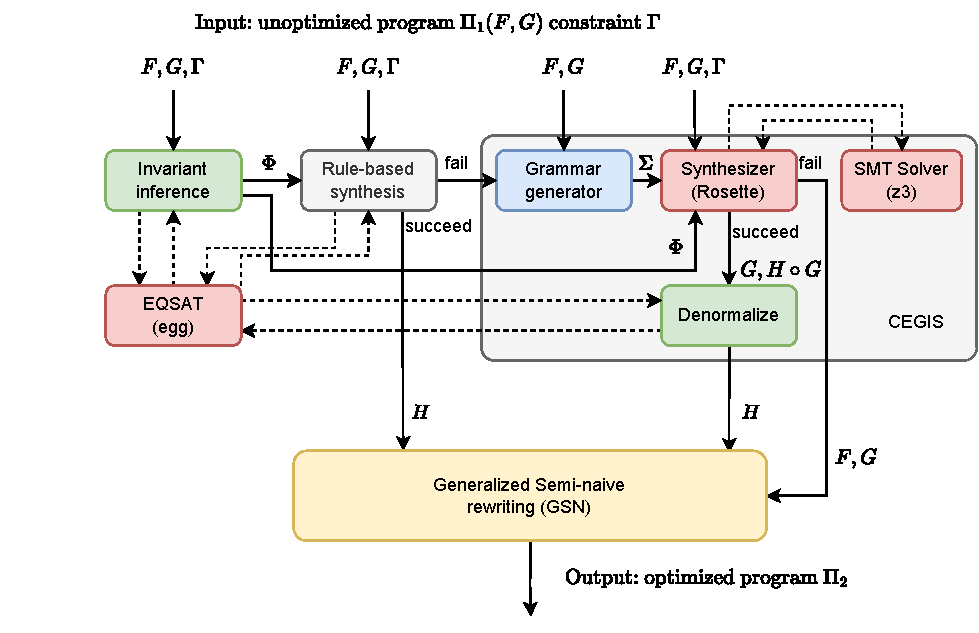
\includegraphics[width=\linewidth]{fgh-optimizer-architecture}
  \caption{The architecture of the FGH-optimizer.  The input is the
    unoptimized program $\Pi_1$, consisting of the functions $F, G$ and
    the database constraint $\Gamma$. The output consists of the
    optimized program $\Pi_2$, see Eq.~\eqref{eq:p1:p2}.  Blue boxes are
    described in Section~\ref{subsec:synthesis} and the green boxes in
    Section~\ref{sec:semantic-opt}.  The yellow box
    (generalized semi-naive optimization) is described in
    Section~\ref{subsec:simple:examples}.  The red boxes represent
    three state-of-the-art systems: Rosette is a \cegis\ system~\cite{DBLP:conf/asplos/Solar-LezamaTBSS06,DBLP:conf/tacas/TorlakJ07,DBLP:conf/oopsla/TorlakB13}, \zzz\ is
    an SMT solver~\cite{10.1007/978-3-540-78800-3_24}, and EGG is an \eqsat\ system~\cite{DBLP:journals/pacmpl/WillseyNWFTP21}.}\label{fig:arch}
\end{figure}


In the rest of the paper we describe our synthesis-based
FGH-optimizer, whose architecture is shown in Fig.~\ref{fig:arch}.  We
optimize one stratum at a time.  We denote by $\Pi_1$ one stratum of
the input program, denote by $X$ its recursive IDBs, by $Y$ its output
IDBs, and by $F,G$ the ICO and the output operator respectively; see
Eq.~\eqref{eq:p1:p2}.  The optimizer also takes as input a database
constraint, $\Gamma$.  The optimizer starts by inferring the loop
invariant $\Phi$; this is discussed in Sec.~\ref{sec:semantic-opt}.
Next, the optimizer needs to find $H$ such that
$\Gamma \wedge \Phi \models \left(G(F(X)) = H(G(X))\right)$.  To
reduce clutter we will often abbreviate this to
$\Gamma \models \left(G(F(X)) = H(G(X))\right)$, assuming that
$\Gamma$ incorporates $\Phi$.  The optimizer makes two attempts at
synthesizing $H$: it first tries using a simpler rule-based
synthesizer, and, if that fails, then it tries the state-of-the-art
Counterexample-Guided Inductive Synthesis (\cegis).  This is described
in Sec.~\ref{subsec:synthesis}.  Finally, $H$ (or the original program
if the FGH-optimization failed) is further transformed using
generalized semi-naive optimization, as we already described in
Sec.~\ref{subsec:simple:examples}.  Notice that stratification ensures
that no interpreted functions are applied to the IDBs $X$; they can
still be applied to the EDBs, or occur in predicates.

The FGH-optimization is an instance of {\em query rewriting using
  views}~\cite{DBLP:journals/vldb/Halevy01,DBLP:conf/sigmod/GoldsteinL01}.
Denoting by $Q \defeq G(F(X))$ and $V \defeq G(X)$, one has to rewrite
the query $Q$ using the view(s) $V$, in other words $Q = H(V)$.  This
is a {\em total} rewriting, in the sense that $H$ may no longer 
refer to the IDBs $X$.  This problem is NP-complete for UCQs with
set semantics~\cite{DBLP:conf/pods/LevyMSS95}, in NP for UCQs with bag
semantics\footnote{This follows from the fact that, under bag semantics, two UCQ queries are
  equivalent iff they are
  isomorphic.~\cite{DBLP:conf/icdt/Green09,DBLP:journals/pvldb/WangHSHL20}.},
and undecidable for realistic SQL queries that include aggregates and
arithmetic~\cite{DBLP:conf/sigmod/GoldsteinL01}.
%
Systems that support query rewriting using views are rule-based, and
apply a set of hand crafted, predefined patterns; our first attempt to
synthesize $H$ is also rule-based.  Such synthesizers usually cannot take advantage
of database constraints, but we will show in
Sec.~\ref{sec:semantic-opt} how to exploit the constraint $\Gamma$ in
the rule-based synthesizer.  However, rule-based rewriting explores a
limited space, which is insufficient for many FGH-optimizations.
In a seminal paper~\cite{DBLP:conf/asplos/Solar-LezamaTBSS06}
Solar{-}Lezama proposed an alternative to rule-based transformation,
called {\em Counterexample-Guided Inductive Synthesis}, \cegis: the
synthesizer produces potentially incorrect candidates, and an SMT
solver verifies their correctness.  In the FGH-optimizer we use a
program synthesizer, Rosette~\cite{DBLP:conf/oopsla/TorlakB13}, to synthesize $H$.

At a conceptual level, program synthesis has two abstract steps: {\em
  generate} $H$, and {\em verify} $G(F(X))=H(G(X))$.  While the
verifier is not used explicitly, it is used implicitly in the
synthesizer, and we describe it in Sec.~\ref{sec:verification}.  Then we
describe the synthesizer in Sec.~\ref{subsec:synthesis}.


% Our optimizer also uses three state of the art tools
% from verification and programming languages: \zzz\ for model checking,
% Rosette for program synthesis, and EGG for equality saturation.  We
% describe them in sections~\ref{sec:verification},
% ~\ref{subsec:synthesis}, and \ref{?????} respectively.


% Any query optimizer can be seen as a theorem prover, capable of
% proving the equivalence of its input and output. From this perspective,
% the rewrite rules in traditional optimizers can be seen as
% {\em axioms}, and the chain of program transformations done by the optimizer
% following these axioms is a calculational proof of equivalence.
% The optimizer's ability to explore alternatives translates to
% its ability to prove programs equal.
% Following this line of thinking, we first demonstrate how to
% {\em verify} the FGH-rule holds. That is, given $F, G$ and $H$,
% we verify $\forall X . G(F(X)) = H(G(X))$.
% Then, building on this verification procedure, we {\em synthesize}
% the function $H$ given $G$ and $F$.


%%% Local Variables:
%%% mode: latex
%%% TeX-master: "main"
%%% End:

\section{Verification}
\label{sec:verification}

\update{
%
  We introduced the FGH-rule in Sec.~\ref{sec:fgh} and showed several
  examples.  In order to apply the rule, one needs to check the
  identity~\eqref{eq:fgh}, $F(G(X))=G(H(X))$. In this section we
  describe how we verify this identity.
%
}
%
This step is implicit in both boxes {\em Rule-based Synthesis} and
\cegis\ in Fig~\ref{fig:arch}.
%
\update{
%
  The identity can be checked in one of two ways: by applying a
  predefined set of identity rules (as currently done by most query
  optimizers), or by using an SMT solver.
%
}

\subsection{Rule-based  Test}\label{sec:axiomatic-rewrite}
% This test consists of first normalizing both expressions, then
% checking for isomorphism.  We describe the rule-based test assuming
% there is no database constraint $\Gamma$: the extension to $\Gamma$
% can be done using a \eqsat\ system, discussed in
% Sec.~\ref{sec:semantic-opt}.


% to handle interpreted functions.
% To simplify implementation, we preprocess the input
%  Datalog program by mapping all semirings in the program to
% the semiring used in $G$.
% For example, the boolean semiring in $CC_{1}$ is mapped to
% the Tropical semiring as shown in Figure~\ref{fig:cc1:semiring}.
% Unifying to a single semiring saves us from enumerating
% tedious axioms describing how different semirings interact
% with each other, and also simplifies the encoding to SMT
% expressions.
%
Let $P_{1} = G(F(X))$, $P_{2} = H(G(X))$.  To check $P_1=P_2$, the
{\em rule-based test} first normalizes both expressions into a
sum-sum-product expression (Eq.~\eqref{eq:sum:sum:product})
via the semiring axioms, then checks if the expressions are isomorphic:
if yes, then $P_{1} = P_{2}$, otherwise we assume $P_{1}\neq P_{2}$.
The treatment of  a constraint $\Gamma$ will be discussed in Sec.~\ref{sec:semantic-opt}.
This test can be visualized as follows:
%
\begin{align}
  P_{1} \xrightarrow[]{\text{axioms}} \text{normalize}(P_{1})
  \simeq
  \text{normalize}(P_{2}) \xleftarrow[]{\text{axioms}} P_{2}
\label{eq:equality:isomorphism}
\end{align}
%
where $\simeq$ denotes isomorphism.  The Rule-based test is sound.
%i.e., there are no false positives.
When both $P_1, P_2$ are over the
$\N^\infty$ semiring and have no interpreted functions then it
is also
complete~\cite{DBLP:conf/icdt/Green09,DBLP:journals/pvldb/WangHSHL20}.
%
This simple test motivates the need for a complete set of axioms that
allows any semiring expression to be normalized.  The axioms include
standard semiring axioms, and axioms about summations and free
variables \texttt{fv}.  For example, in order to
prove $CC_1 = CC_2$ in Example~\ref{ex:fgh:cc} (with
semiring notation in Figure~\ref{fig:cc1:semiring}) one needs
all three axioms below:
%
\begin{align}
  \bigoplus_x \bigoplus_y \left(\cdots\right) = \ &  \bigoplus_{x,y}\left( \cdots \right)  \label{eq:axiom:plus:plus} \\
  A \otimes \bigoplus_{x} B = \ & \bigoplus_{x} A \otimes B \text{ when } x \not \in \texttt{fv}(A) \label{eq:axiom:pullmul}\\
  \bigoplus_x \left(A(x) \otimes [x=y]\right) = \ & A(y)  \label{eq:axiom:plus:equal}
\end{align}
%

%
%
%
%
% \begin{example} We illustrate how to check of the FGH-rule in
%   Example~\ref{ex:fgh:cc}.  The two expressions $P_1, P_2$ were denote
%   $CC_1, CC_2$ and are shown in Figures~\ref{fig:cc1}
%   and~\ref{fig:cc2}.  We first de-sugar them and write them as
%   semiring expressions, as shown in Figure~\ref{fig:cc1:semiring}.
%   Recall that the cast operator $[-]_\infty^0$ maps the Boolean values
%   $0,1$ to the tropical values $\infty, 0$. We normalize both
%   expressions, using semiring axioms such as:
% %
%   \begin{align}
%     \bigoplus_x \bigoplus_y \left(\cdots\right) = &  \bigoplus_{x,y}\left( \cdots \right)  \label{eq:axiom:plus:plus} \\
%     A \otimes \bigoplus_{x} B = & \bigoplus_{x} A \otimes B \text{ when } x \not \in \texttt{fv}(A) \label{eq:axiom:pullmul}\\
%     \bigoplus_x \left(A(x) \otimes [x=y]\right) = & A(y)  \label{eq:axiom:plus:equal}
%   \end{align}
% %
%   We have designed a complete set of semiring axioms for converting
%   into a sum-sum-product expression, similar to axioms found
%   elsewhere,
%   e.g., \cite{DBLP:journals/pvldb/ChuMRCS18,DBLP:journals/pvldb/WangHSHL20}.
%   After normalization, we obtain:
% %
%   \begin{align*}
%     \text{normalize}(CC_{1}[x]) & = L[x] \oplus \bigoplus_{y,z} L[y] \otimes \totrop{E(x,z)} \otimes [TC(z,y)]_{\infty}^{0}\\
%                                 & \simeq \text{normalize}(CC_{2}[x])
%   \end{align*}
% %
%   proving their equivalence.
% %   Each rewrite step during normalization applies some semiring axioms,
% %   for example: where $\texttt{fv}(A)$ is the set of free variables in
% %   $A$.  We use standard semiring identities like the commutativity and
% %   associativity of $\oplus$ and $\otimes$ in the normalization step.
% %   We omit the exhaustive list of axioms, and refer the reader
% %   to~\cite{??} for details.
% \end{example}
%

% In some cases this mapping is lossless;
% for example boolean disjuction $x \vee y$ can be mapped
% via inclusion-exclusion to $[x] + [y] - [x] \times [y]$,
% where $[\cdot]$ casts \texttt{true} to $1$ and
% \texttt{false} to $0$.
% In other cases this mapping is lossy.
% For example we map $\min(x,y)$ to $x+y$,
% however $\min(x,x) = x$ but $x+x \neq x$.
% In general, mapping to the sum-product semiring is always
% sound:
% \begin{theorem}[Equality over $(\N, +, \times, 0, 1)$ is canonical]\label{th:soundness}
%   $[e_{1}]_{\N} = [e_{2}]_{\N} \Rightarrow e_{1} = e_{2}$,
%   where $e_{1}$ and $e_{2}$ are over the same semiring, and
%   $[\cdot]_{\N}$ maps an expression in any semiring to the sum-product semiring.
% \end{theorem}
% We note that it is possible, albeit tedious, to skip this
% processing step and apply axioms specific to each semiring,
% and to directly encode each semiring in SMT formulas.
% An industrial-strength optimizer may opt to do so to achieve
% better coverage.
\begin{figure}
% \fcolorbox{black}{light-gray}{\parbox{0.2\textwidth}{
  \begin{align*}
    CC_{1}[x] & = \bigoplus_{y} L[y] \otimes \big([x=y]_{\infty}^{0} \oplus \bigoplus_{z} [E(x,z)]_{\infty}^{0} \otimes [TC(z,y)]_{\infty}^{0}\big) \\
    CC_{2}[x] & = L[x] \oplus \bigoplus_{y} \big( \bigoplus_{y'} L[y'] \otimes [TC(y,y')]_{\infty}^{0}\big) \otimes [E(x,y)]_{\infty}^{0}
  \end{align*}
% }}
  \caption{$CC_{1}$ and $CC_{2}$ in semiring notation; their normal
    forms are isomorphic.}
  \label{fig:cc1:semiring}
\end{figure}
% \begin{figure}
% \fcolorbox{black}{light-gray}{\parbox{0.2\textwidth}{
% \footnotesize
%   \begin{align*}
%     CC_{2}[x] \defeq L[x] \oplus \bigoplus_{y} 1_{E(x,y)} \otimes \bigoplus_{y'} L[y'] \otimes 1_{TC(y,y')}
%   \end{align*}
% }}
%   \caption{$CC_{2}$ in semiring notation.}
%   \label{fig:cc2:semiring}
% \end{figure}

\subsection{SMT Test} \label{subsubsec:smt:test} When the
expressions $P_1, P_2$ are over a semiring other than $\N^\infty$, or
they contain interpreted functions, then the rule-based test is
insufficient and we use an SMT solver for our verifier.
We still normalize the
expressions using our axioms, because today's solvers cannot reason
about bound/free variables (as needed in
axioms~\eqref{eq:axiom:plus:plus}-\eqref{eq:axiom:plus:equal}).  The
{\em SMT test} is captured by the following figure:
% After we normalize both expressions
% $P_{1}$ and $P_{2}$, if the isomorphism test fails, then we check
% their equivalence using an SMT solver: $\Gamma \models (P_1=P_2)$.
% More precisely, we ask the solver to find a {\em counterexample}, i.e.,
% IDB and EDB instances for which
% $\Gamma \wedge (\text{normalize}(P_1)\neq \text{normalize}(P_2))$.  If
% the solver fails, i.e., returns \textsf{UNSAT}, then we know that
% $P_1 = P_2$.  The following figure captures this process:
%
%
% If the equality is
% valid, $P_{1}$ and $P_{2}$ are equivalent; otherwise they are not, and
% the solver will return a {\em counterexample} input to $P_{1}$ and
% $P_{2}$ on which they evaluate to different results.  We illustrate
% this process as follows:
\begin{align}
  P_{1} \xrightarrow[]{\text{axioms}} \text{normalize}(P_{1})
  \xleftrightarrow{\text{SMT}} &
  \text{normalize}(P_{2}) \xleftarrow[]{\text{axioms}} P_{2} \label{eq:equality:smt}
\end{align}

\begin{ex}[APSP100]\label{ex:sssp100}
  Consider a labeled graph $E$ where $E[x,y]$ represents the cost of
  the edge $x,y$.  The following query over $\trop$
  computes the all-pairs shortest
  path up to length of 100:
%
{
  \begin{align}
    D[x,y] \cd & \texttt{if } x=y \texttt{ then } 0 \texttt{ else } \min_{z} \left(D[x,z] +E[z,y]\right) \nonumber \\
    Q[x,y] \cd & \min(D[x,y],100)  \label{eq:apss:opt}
  \end{align}
}
%
  % The first rule is not {\em safe}, because $x$ does not occur in
  % relational atom; one can convert it to a safe rule by restricting
  % $x$ to range over the set of nodes in the graph, but we omit that in
  % order to reduce clutter.  The second rule is both recursive {\em
  %   and} contains an aggregate operator, $\min$.  If one were to
  % represent it in standard Datalog, it would be something like this:
%
  % \begin{align*}
  %   D(x,y,\min(v+c)) \cd & D(x,z,v),E(z,y,c)
  % \end{align*}
%
  % In standard  Datalog rules with aggregates are not monotone.  In
  % order to add such rules to Datalog, prior
  % work~\cite{DBLP:conf/pods/GangulyGZ91,DBLP:journals/tkde/SeoGL15}
  % has re-defined the semantics of the $\min$ operator, whenever it
  % occurs in the head of a recursive rule.  Instead, in $\name$ our
  % approach is to use a standard semantics, by generalizing from the
  % Boolean semiring to an arbitrary ordered semiring.  The
  % program~\eqref{eq:apss:opt} is interpreted over the tropical
  % semiring $\trop = (\N \cup \set{\infty},\min,+,\infty,0)$.  The
  % program is monotone and has a unique least fixpoint.
  The program is inefficient because it first computes the full path
  length, only to cap it later to 100.  By using the FGH-rule we get:
%
{
  \begin{align}
    Q[x,y] \cd & \texttt{if } x=y \texttt{ then } 0 \texttt{ else } \min\left(\min_{z} \left(Q[x,z]+E[z,y]\right),100\right) \label{eq:apss:opt:opt}
  \end{align}
}
%
We show how to verify
that~\eqref{eq:apss:opt:opt} is equivalent to~\eqref{eq:apss:opt}.
Denote by $P_1 \defeq G(F(D))$ and $P_2 \defeq H(G(D))$ (where $F,G,H$
are the obvious functions in the two programs defining $Q$).  After we
de-sugar, convert to semiring expressions, and normalize,
they become:
%
{
\begin{alignat*}{2}
  P_{1}[x,y] & =  \left(0 \otimes \totrop{x=y}\right) \oplus \left(\bigoplus_{z} D[x,z] \otimes E[z,y]\right) && \oplus 100 \\
  P_{2}[x,y] % & = 0 \otimes \totrop{x=y} \oplus 100 \oplus \bigoplus_{z} (D[x,z] \oplus 100) \otimes E[z,y] \\
             % & = 0 \otimes \totrop{x=y} \oplus 100 \oplus \bigoplus_{z} D[x,z] \otimes E[z,y] \\
             % & \hskip 59pt \oplus \bigoplus_{z} 100 \otimes E[z,y] \\
%              & = 100 \oplus 0 \otimes \totrop{x=y} \oplus \bigoplus_{z} D[x,z] \otimes E[z,y] \\
%              & \hskip 25pt \oplus 100 \otimes \bigoplus_{z} E[z,y] \\
             & = \left(0 \otimes \totrop{x=y}\right) \oplus \left(\bigoplus_{z} D[x,z] \otimes E[z,y]\right) && \oplus \left(100 \otimes\bigoplus_{z} E[z,y]\right) \\
             &&& \oplus 100
\end{alignat*}
}
%
In the normalized expressions we push the summations past the joins,
i.e., we apply rule~\eqref{eq:axiom:pullmul} from right to left, thus
we write $100 \otimes \bigoplus (\cdots)$ instead of
$\bigoplus (100 \otimes \cdots)$: we give the rationale below.  At
this point, the normalized $P_{1}$ and $P_{2}$ are not isomorphic, yet
they are equivalent if they are interpreted in $\trop$.
We explain below in detail how the solver can check that.
In this particular semiring,
the
identity
$
  100 = \left(100 \otimes \bigoplus_{z} E[z,y]\right)  \oplus 100
$
holds since it becomes
$
100 = \min(100 + \min_{z} E[z,y],100)
$
with $E[z,y] \geq 0$,
once we replace the uninterpreted operators
$\oplus, \otimes$ with $\min, +$.
%
% As we explain below, an SMT solver can prove this identity given that
% $E[z,y] \geq 0$.  More precisely, using the \zzz\ solver, we discover
% that the following is \textsf{UNSAT}:
% \[
% x \geq 0 \wedge 100 \neq \min(100 + x, 100)
% \]
% from which we can conclude
% $\forall x . x \geq 0 \Rightarrow 100 = \min(100, 100 + x)$.
\end{ex}


{\bf Implementation} We describe how we implemented the SMT test
$\Gamma \models P_1 = P_2$ using a solver, now also taking
the database constraint $\Gamma$ into account, where
$P_1, P_2$ are the expressions $G\circ F$
and $H \circ G$. We used the \zzz\ solver~\cite{10.1007/978-3-540-78800-3_24}, but our
discussion applies to other solvers as well. We need to normalize
$P_1, P_2$ before using the solver, because solvers require all axioms
to be expressed in First Order Logic. They cannot encode the
axioms~\eqref{eq:axiom:plus:plus}-\eqref{eq:axiom:plus:equal}, because
they are referring to free variables, which is a
meta-logical condition not expressible in First Order Logic.
Once normalized, we encode the equality as a first-order logic
formula, and assert its negation, asking the solver to check if
$\Gamma \wedge \left(P_1 \neq P_2\right)$ is satisfiable.  The solver
returns $\textsf{UNSAT}$, a counterexample, or
$\textsf{UNKNOWN}$.  $\textsf{UNSAT}$ means the
identity holds.  When it returns a counterexample, then the identity
fails, and the counterexample is given as input to the synthesizer
(Sec.~\ref{subsec:synthesis}).  $\textsf{UNKNOWN}$ means that it could
neither prove nor disprove the equivalence and we
assume $P_1 \neq P_2$.  For the theory of reals with $+, *$, despite its
decidability,  \zzz\ often timed out in our experiments.
We therefore used the theory of integers, and
\zzz\ never timed out or returned $\textsf{UNKNOWN}$ in our experiments.



We encode every $\bm S$-relation
$R(x_1, \dots, x_n)$ as an uninterpreted function
$R : \N \times \cdots \times \N \rightarrow \bm S$, where $\bm S$ is
the {\em interpreted} semiring, i.e., $\B$, $\trop$, $\N^\infty$, etc.
We represent natural numbers as
integers with nonnegativity assertions, and represent
the sets $\N^\infty, \N_\bot, \R_\bot$ as union types.
Operators supported by the solver, like $+, *, \min, -$,
are entered unchanged; we treat other operators
as uninterpreted functions.  Unbounded aggregation, like
$\bigoplus_{x} e(x)$, poses a challenge:  there is no
such  operation in any SMT theory.
%%% One may attempt to unfold
%%% the aggregate over some bounded values of $x$, say replace
%%% $\min_{x} e(x)$ with $\min(e(0), \dots, e(20))$, but this approach is
%%% unsound.
Here we use the fact that $P_1$ and $P_2$ are normalized
sum-sum-product~expressions:
%
\begin{align*}
P_1 = & \left(\bigoplus_{x_1} e_1\right) \oplus \left(\bigoplus_{x_2}  e_2\right) \oplus \cdots
&
P_2 = & \left(\bigoplus_{x_1'} e_1'\right) \oplus \left(\bigoplus_{x_2'} e_2'\right) \oplus \cdots
\end{align*}
%
Assume first that each $x_i$ is a single variable. We
ensure that all the variables $x_1, x_2, \ldots$ in $P_1$ are
distinct, by renaming them if necessary.  Next, we replace each
expression $\bigoplus_{x_i} e_i$ with $u(x_i,e_i)$ where $u$ is an
uninterpreted function.  Finally, we ask the solver to check
%
\begin{align}
\Gamma \models \left(u(x_1,e_1) \oplus u(x_2,e_2) \oplus \cdots =  u(x_1',e_1') \oplus u(x_2',e_2') \oplus \cdots\right)
\nonumber
% \label{eq:ui:uj}
\end{align}
%
This procedure is sound, because if the identity $u(x,e) = u(x',e')$
holds, then $x=x'$ (they are the same variable) and $e=e'$, which
means that $\bigoplus_x e = \bigoplus_{x'} e'$.  Moreover,
when synthesizing $P_2$, we will
ensure that the generator includes the variables $x_1, x_2, \ldots$
present in $P_1$ to achieve a limited form of completeness,
see
Sec.~\ref{subsec:synthesis}. Finally, if a
summation is over multiple variables, we simply nest the uninterpreted
function, i.e., write $\bigoplus_{x,y} e$ as $u(x,u(y,e))$.

\begin{ex}  We now finish Example~\ref{ex:sssp100}.
After introducing the
  uninterpreted functions described above, we obtain:
%
  \begin{align*}
    P_1 = & \min(0+w(x,y), u(z,D[x,z]+E[z,y]), 100) \\
    P_2 = & \min(0+w(x,y), u(z,D[x,z]+E[z,y]), 100+u(z,E[z,y]), 100)
  \end{align*}
  where $w(x,y)$ is an uninterpreted function representing
  $[x=y]_\infty^0$, and $u$ is our uninterpreted function encoding
  summation.  The solver proves that the two expressions are equal,
  given that $w \geq 0$ and $u \geq 0$.  Notice that it was critical
  to factorize the term 100: had we not done that, then the expression
  $100+u(z,E[z,y])$ would be $u(z,100 + E[z,y])$ and the identity
  $P_1=P_2$ no longer holds.
\end{ex}

\required{
%
  {\bf Discussion} Readers unfamiliar with First Order Logic may be
  puzzled by our statement that the identity $u(x,e)=u(x',e')$ holds
  iff $x=x'$ and $e = e'$.  In order to explain this, it helps to
  first review the basic definitions of validity and satisfiability in
  logic.  A statement is ``valid'' if it is true for all
  interpretations of its uninterpreted symbols.  For example, the
  equality $f(x)+y=y+f(x)$ is valid over integers, because it holds
  for all function $f$ and all values of $x$ and $y$.  A statement is
  ``satisfiable'' if there exists interpretations of its uninterpreted
  symbols that make the statement true.  A statement is valid iff its
  negation is not satisfiable.  In our case, the statement
  $u(x,e)=u(x',e')$ is valid if the equality is true for all possible
  interpretations of $u, x, x'$.  For example, suppose we asked the
  solver to check whether $u(x,2(x+1)) = u(y,2y+2)$ is valid.  To
  answer this question, we negate the statement and ask the \zzz\
  solver whether the negation is satisfiable:
  $u(x,2(x+1))\neq u(y,2y+2)$.  One can easily satisfy this with pen
  and paper, e.g.,  $x=1, y=2, u(a,b)=a+b$, then $u(x,2(x+1))=5$,
  $u(y,2y+2)=8$.  \zzz\ also answers ``yes'', and provides the
  following example for the inequality\footnote{Please refer to the
    documentation of \zzz\ for how models for uninterpreted functions
    are constructed.}:
  \[x=0, y=38, u(a,b)= \text{if } a=38\wedge b=78 \text{ then } 6 \text{ else } 4\]
  Therefore, the identity $u(x,2(x+1)) = u(y,2y+2)$ is not valid.  In
  contrast, suppose we asked the solver whether
  $u(x,2(x+1)) = u(x,2x+2)$ is valid.  Its negation is
  $u(x,2(x+1)) \neq u(x,2x+2)$, and \zzz\ returns $\textsf{UNSAT}$,
  which means that the identity is valid.  In general, the identity
  $u(x,e)=u(x',e')$ is valid iff $x=x'$ and $e=e'$.
%
}


% \reinhard{uniform notation: $p_1$ and $p_2$ vs. $P_1$ and $P_2$?}
% \dan{done; hope  i didn't missed anything}

% This encoding of aggregates is complete
% in the following sense:
% %
% \begin{theorem}[Encoding $\bigoplus$ with uninterpreted functions]
%   $\bigoplus_{x} e = \bigoplus_{x'} e' \Leftrightarrow f_{\bigoplus}(x, e) = f_{\bigoplus}(x',e')$
%   where $\bigoplus_{x} e$ and $\bigoplus_{x'} e'$ are in normal form.
% \end{theorem}
% %
% The following shows the SMT encoding of $Q_{1}$ and $Q_{2}$:
% \begin{align*}
%   Q_{1} & : \min(100, 0 + \totrop{x=y}, f_{\min}(z, f_{D}(x,z) + f_{E}[z,y])) \\
%   Q_{2} & : \min(100, 0 + \totrop{x=y}, f_{\min}(z, f_{D}(x,z) + f_{E}[z,y]), \\
%         & \hskip 26pt 100 + f_{\min}(z, f_{E}[z,y]))
% \end{align*}

%%% \subsubsection{Discussion} In summary, our verifier checks $p_1 = p_2$
%%% by first normalizing both expressions, checking for isomorphism,
%%% \eqref{eq:equality:isomorphism} and, if that fails, then using the
%%% \zzz\ solver to check their equivalence, \eqref{eq:equality:smt}.  The
%%% reader may wonder why we don't bypass normalization altogether and
%%% perform the entire verification pipeline in the solver.  The reason is
%%% that the solver requires all axioms to be expressed in First Order
%%% Logic, while some crucial axioms needed for identities of
%%% sum-sum-product expressions require checking for free variables, as in
%%% example~\eqref{eq:axiom:pullmul}, which is a meta-logical condition,
%%% and not expressible in First Order Logic.  In other words, we are
%%% extending the solver with specialized knowledge about the semiring.

%
% Moreover, other axioms
% expressible in FOL usually require quantification and can easily make
% SMT-solving undecidable or intractable. \dan{I don't understand the
%   last sentence}

% In summary, the verification process first normalizes the pair of expressions
% to be checked.
% If the normal forms are isomorphic, the expressions are equivalent and verification succeeds.
% Otherwise, we encode the expressions in an SMT formula that asserts their equivalence,
% then checks the validity of this formula with an SMT solver.
% The entire pipeline looks like the following:

%%% Local Variables:
%%% mode: latex
%%% TeX-master: "main"
%%% End:

\section{Synthesis}

\label{subsec:synthesis}

%%% \dan{currently: 1.5 pages.  GOAL: 1 PAGE.  Reinhard: the section is
%%%   complete, but can use lots of polishing, feel free to edit it.}

\update{
%
We have seen in Sec.~\ref{sec:verification} how to use an SMT solver
to check the identity $G(F(X))=H(G(X))$.
%
}
%
We are now ready to discuss the core of the FGH-optimizer: given 
the query expressions $F, G$, find $H$ such that the
identity $G(F(X)) = H(G(X))$ holds; recall that we denote these
expressions by $P_1, P_2$. As for verification, this can be done by
using only rewriting, or using program synthesis with an SMT solver.
We are also given a database constraint $\Gamma$, and we assume that
 we have already added to it the loop invariant $\Phi$.


\subsection{Rule-based Synthesis}
\label{subsec:rule:based:synthesis}

The optimizer first attempts to synthesize $H$ using rule-based
rewriting.  This process is akin to our initial verifier that relies
only on normalization and isomorphism checking.
%
\begin{align}
  P_{1} \xrightarrow[]{\text{axioms}} \text{normalize}(P_{1}) \xrightarrow[]{\text{axioms}} P_{2}
  \label{eq:synthesis:isomorphism}
\end{align}
%
There is no obvious way to ``denormalize'' an expression, since many
expressions share the same normal form.  We used for this purpose
an equality saturation system (\eqsat), also used for multiple tasks
of the FGH-optimizer, see Fig~\ref{fig:arch}.  We describe \eqsat\ in Sec.~\ref{sec:semantic-opt}.
% One possibility is to apply one of the query rewriting using views
% algorithms, like MiniCon~\cite{DBLP:journals/vldb/PottingerH01} or
% pattern-matching as used in SQL
% Server~\cite{DBLP:conf/sigmod/GoldsteinL01}.  Instead, we use for
% this purpose an equality saturation system, described in
% Sec.~\ref{sec:semantic-opt}.

% \reinhard{Can we give a short justification for our decision to use
% an equality saturation system?}


%%% Instead, we chose to use for this purpose a state of the art {\em
%%%   equality saturation} system (\eqsat) developed in the programming
%%% language community, called
%%% EGG~\cite{DBLP:journals/pacmpl/WillseyNWFTP21}.  Using an open source
%%% \eqsat\ system simplifies considerably the development of our
%%% optimizer, but, conceptually, it does not bring anything new to {\em
%%%   this task} over what was previously known in the literature, so we
%%% delay its description to Sec.~\ref{sec:semantic-opt}.

% A brute-force approach is
% to rewrite the input $P_{1}'$ to as many equivalent expressions as
% possible, and then look for an expression of the form $H(G(X))$ among
% the results.  This naive idea is implemented efficiently by an
% innovation in programming languages dubbed {\em equality saturation}
% (\eqsat).



\subsection{Counterexample-based Synthesis}

The rule-based synthesis~\eqref{eq:synthesis:isomorphism} explores
only correct rewritings $P_2$, but its space is limited by the
hand-written axioms. The alternative approach, pioneered in the
programming language
community~\cite{DBLP:conf/asplos/Solar-LezamaTBSS06}, is to synthesize
candidate programs $P_2$ from a much larger space, then using an SMT
solver to verify their correctness.  This technique, called
Counterexample-Guided Inductive Synthesis, or \cegis, can find
rewritings $P_2$ even in the presence of interpreted functions,
because it exploits the theory of the underlying domain.  As a first
attempt it can be described as follows (we will revise it below):
%
\begin{align}
  P_{1} \xrightarrow[]{\text{axioms}} \text{normalize}(P_{1}) \xrightarrow[]{\cegis} P_{2}
  \label{eq:synthesis:cegis}
\end{align}
%

\subsubsection{Brief Overview of \cegis} We give a brief overview of
the \cegis\ system,
Rosette~\cite{DBLP:conf/tacas/TorlakJ07,DBLP:conf/oopsla/TorlakB13},
that we used in our optimizer.  Understanding its working is
important in order to optimize its usage for FGH-optimization.  The
input to Rosette consists of a {\em specification} and a {\em
  grammar}, and the goal is to synthesize a program defined by the
grammar and that satisfies the specification.
% The \cegis\ algorithm is illustrated by Figure~\ref{fig:cegis}.
The main loop is implemented with a pair of {\em dueling} SMT-solvers,
the {\em generator} and the {\em checker}.  In our setting, the inputs
are the query $P_1$, the database constraint $\Gamma$, and a small
grammar $\Sigma$ (described below).  \update{The specification is
  $\Gamma \models (P_1 = P_2)$, where $P_2$ is defined by the grammar
  $\Sigma$.}  The generator generates syntactically correct programs
$P_2$, and the verifier checks $\Gamma \models (P_1 = P_2)$.  In the
most naive attempt, the generator could blindly generate candidates
$P_2, P_2', P_2'', \ldots$, until one is found that the verifier
accepts.  This is hopelessly inefficient.  The first optimization in
\cegis\ is that the verifier returns a small counterexample database
instance $D$ for each unsuccessful candidate $P_2$, i.e.,
$P_1(D)\neq P_2(D)$.  When considering a new candidate $P_2$, the
generator checks that $P_1(D_i) = P_2(D_i)$ holds for all previous
counterexamples $D_1, D_2, \ldots$, by simply evaluating the queries
$P_1,P_2$ on the small instance $D_i$.  This significantly reduces the
search space of the generator.

\cegis\
applies a second optimization, where it uses the SMT solver itself to
generate the next candidate $P_2$, as follows.  It requires a fixed
recursion depth for the grammar $\Sigma$; in other words we can assume
w.l.o.g. that $\Sigma$ is non-recursive.  Then it associates a
symbolic Boolean variable $b_1, b_2, \ldots$ to each choice of the
grammar.  The grammar $\Sigma$ can be viewed now as a BDD (binary
decision diagram) where each node is labeled by a choice variable
$b_j$, and each leaf by a completely specified program $P_2$.  The
search space of the generator is now completely defined by the choice
variables $b_j$, and Rosette uses the SMT solver to generate values
for these Boolean variables such that the corresponding program $P_2$
satisfies $P_1(D_i) = P_2(D_i)$, for all counterexample instances
$D_i$.  This significantly speeds up the choice of the next candidate
$P_2$.


% The \eqsat-based optimization of pure $\name$ can be
% understood in parallel to the normalization-based verification
% process: both rely on axiomatic rewrites of the input expressions.
% Similarly, our optimizer for $\name$ with interpreted functions
% builds on the solver-aided verification procedure.
% In verifying the FGH-rule we start from the expressions
% $G(F(X))$ and $H(G(X))$ and ``meet in the middle'';
% the optimization problem requires us to start from the initial
% program $G(F(X))$ and arrive at the optimized program $H(G(X))$.
% We summarize our query synthesis pipeline as follows:
% \[
%   G(F(X)) \xrightarrow[]{\text{axioms}} \text{normalize}(P_{1})
%   \xrightarrow[]{\cegis}
%   P_{2}' \xrightarrow[]{\eqsat} H(G(X))
% \]
% We first normalize the input program $G(F(X))$
% to $\text{normalize}(P_{1})$ by applying semiring axioms.
% Then we leverage counterexample-guided inductive synthesis (\cegis),
% a novel technique from programming languages,
% to synthesize $P_{2}'$ such that $ P_{2}' = \text{normalize}(P_{1})$;
% furthermore, $P_{2}'(X)$ must be the normal form of $H(G(X))$ for some $H$.
% Finally, we denormalize $P_{2}'(X)$ into $H(G(X))$ with \eqsat\
% and extract the optimized recursive definition $H$.

% \subsubsection{Query synthesis with \cegis}

% \begin{figure}
%   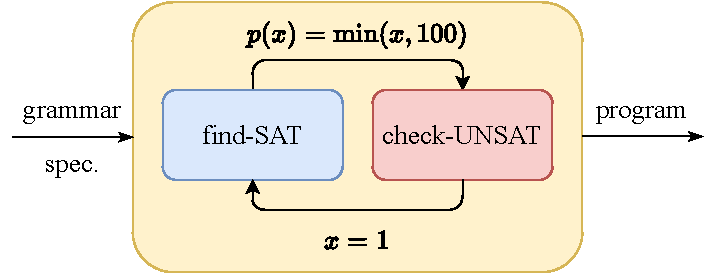
\includegraphics[width=0.8\linewidth]{duel}
%   \caption{Architecture of \cegis.}\label{fig:cegis}
% \end{figure}

% \cegis~takes a grammar $\Gamma$ and a specification $\psi$,
% and outputs a program $p$ drawn from $\Gamma$ that satisfies $\psi$.
% $\psi$ is a first-order formula where the input variables to $p$
% are $\forall$-quantified;
% $\Gamma$ is a conjunction of implications,
% where each implication specifies one alternative in the grammar.


% \begin{example}[Simple \cegis\ Problem]\label{ex:simple:cegis}
%   The following specifies a \cegis\ problem
%   to find a $p$ such that $\forall x . 100 = 100 + p(x)$,
% given the grammar $p(x) \coloneqq 100 + x \mid \min(100, x)$.
%   \begin{gather*}
%     \psi \defeq \forall x . 100 = 100 + p(x)\\
%     \Gamma \defeq (b \Rightarrow p(x) = 100 + x) \wedge (\neg b \Rightarrow p(x) = \min(100, x))
%   \end{gather*}
%   Each pair of $b$ and $\neg b$ correspond to
%   a choice operator ``$\mid$'' in the grammar.
%   Note this is the main step checked by the SMT solver
%   in verifying Example~\ref{ex:sssp100}.
% \end{example}

% The essence of the \cegis\ algorithm is illustrated by Figure~\ref{fig:cegis}.
% The main loop is implemented with a pair of {\em dueling} SMT-solvers,
% one called the {\em generator} (in blue)
% and the other the {\em checker} (in red).
% The generator maintains an initially empty set of counterexamples \textsf{CE}.
% At every iteration of the loop, it draws a program from the grammar that
% satisfies $\psi$ on all existing counterexamples.
% To do so, it solves the following formula:
% $$\Gamma \wedge \bigwedge_{v\in \textsf{CE}} \psi(v)$$
% where $\psi(v)$ means to substitute the quantified variable in $\psi$ with $v$.
% For example, given $\Gamma$ and $\psi$ in Example~\ref{ex:simple:cegis}
% with $\textsf{CE} = \{ 0\}$ the generator solves:
% \begin{gather*}
%   \Gamma \defeq (b \Rightarrow p(x) = 100 + x) \wedge (\neg b \Rightarrow p(x) = \min(100, x)) \\
%   \Gamma \wedge x = 0 \wedge 100 = 100 + p(x)
% \end{gather*}
% This is satisfiable by assigning either \texttt{true} or \texttt{false} to $b$;
% suppose the generator binds $b$ to \texttt{false},
% therefore proposing $p(x) = \min(100, x)$ as a candidate solution.
% It sends this candidate to the checker to verify its correctness against $\psi$.
% Upon receiving a candidate $p$, the checker instantiates $\psi$ with it
% and checks the validity of the resulting formula, by solving its negation:
% \begin{gather*}
%   \text{SAT?}\Big(
%   \neg\big(100 = 100 + p(x) \big)
% \Big)
%   \text{ where } p(x) \defeq \min(100, x)
% \end{gather*}
% This is satisfied when $x=1$, so the candidate $p(x) = \min(100, x)$ is not correct.
% The checker then adds $1$ to \textsf{CE} as feedback
% explaining why the candidate is wrong.
% As this generate-check loop continues,
% the proposed candidate will satisfy $\psi$ on more and more inputs.
% When the checker returns \textsf{UNSAT},
% it has found a correct $p$ and outputs it as the solution.
% On the other hand,
% an \textsf{UNSAT} result from the generator indicates the \cegis\ problem has no solution.
% Indeed, the generator would propose the correct $p$ on the next iteration
% on our example problem, because $b$ must be set to \texttt{true}
% to satisfy $\Gamma \wedge \psi(1)$.
%
% To incorporate \cegis\ into our synthesis pipeline,
% we define the specification to be:
% \[
% \psi \defeq \forall X .  \text{normalize}(P_{1})(X) = p(X)
% \]
% The challenge now is to define the grammar $\Gamma$,
% such that any $p(X)$ drawn from $\Gamma$ can be denormalized into $H(G(X))$
% for some $H$.
% We can design such a grammar by analyzing the possible forms $H(G(X))$ may take.

\subsubsection{Using Rosette} To use Rosette, we need to define the
specification and the grammar. A first attempt is to simply define
some grammar for $H$, with the specification
$\Gamma \models \left(G(F(X)) = H(G(X))\right)$.  This does not work,
since Rosette uses the SMT solver to check the identity: as explained
in Sec.~\ref{subsubsec:smt:test}, modern SMT solvers have limitations
that require us to first normalize $G(F(X))$ and $H(G(X))$ before
checking their equivalence.
Even if we modify Rosette
to normalize $H(G(X))$ during verification,
there is still no obvious way to incorporate normalization
into the program generator driven by the SMT solver.
Instead,
we define a grammar $\Sigma$ for $\text{normalize}(H(G(X)))$ rather
than for $H$, and then specify:
\[
\Gamma \models \text{normalize}(G(F(X))) = \text{normalize}(H(G(X)))
\]
Then, we denormalize the result
returned by Rosette, in order to extract $H$, using the {\em
  denormalization} module in Fig.~\ref{fig:arch}, described in
Sec.~\ref{sec:semantic-opt}.  In summary, our \cegis-approach for
FGH-optimization can be visualized as follows:
%
\begin{align}
  P_{1} \xrightarrow[]{\text{axioms}} \text{normalize}(P_{1}) \xrightarrow[]{\cegis} \text{normalize}(P_{2}) \xrightarrow[]{\text{axioms}} P_{2}
  \label{eq:synthesis:cegis2}
\end{align}
%
The choice of the grammar $\Sigma$ is critical for the FGH-optimizer.
If it is too restricted, then the optimizer will be limited too, if it
is too general, then the optimizer will take a prohibitive amount of
time to explore the entire space.  We briefly describe our design at a
high level.  Recall that $X$ denotes multiple IDBs, and the query
$G(X)$ may also return multiple intermediate relations. In our system
$G(X)$ is restricted to return a single relation, so we will assume
that $Y = G(X)$ is a single IDB.  The expression $G$ is known to us,
and is a sum-sum-product expression, see
Eq.~\eqref{eq:sum:sum:product},
%
\begin{align*}
  G(X) = & G_1(X) \oplus \cdots \oplus G_m(X)
\end{align*}
%
where each $G_i(X)$ is a sum-product expression,
Eq.~\eqref{eq:t:mono}, using the IDBs $X$ and/or the EDBs.

To generate $\texttt{normalize}(H(G(X)))$, \update{we group its
  sum-products by the number of occurrences of $Y$:}
%
\begin{align*}
  \texttt{normalize}(H(Y)) = &  H^{(0)} \oplus H^{(1)}(Y) \oplus
  \cdots \oplus H^{(k_{\max})}(Y)
\end{align*}
%
where $H^{(k)}$ is a sum-sum-product
$H^{(k)} = Q_1 \oplus Q_2 \oplus \cdots$ s.t. each $Q_i$ contains
exactly $k$ occurrences of $Y$, and an arbitrary number of EDBs (it
may not contain the IDBs $X$).  We choose $k_{\max}$ as the largest
number of recursive IDBs $X$ that occur in any rule of the original
program $F(X)$, e.g.,  if the original program was linear, then
$k_{\max} \defeq 1$.  We obtain:
%
{
\begin{align*}
  & \texttt{normalize}(H(G(X))) = \\
  & \ \ \ \   H^{(0)} \oplus \texttt{normalize}(H^{(1)}(G(X))) \oplus \cdots \oplus \texttt{normalize}(H^{(k_{\max})}(G(X)))
\end{align*}
}
%
%
The grammar $\Sigma$ is shown in Fig.~\ref{fig:grammar}.  The start
symbol, $A$, generates a sum matching the expression above.  $A_0$
generates $H^{(0)}$, which is a sum of sum-product terms without any
occurrence of $Y$.  Recall from Sec.~\ref{subsubsec:smt:test} that the
expression $u(z,Q)$ denotes $\bigoplus_z Q$.  $E$ is one of the EDBs,
and $Z$ is a non-terminal for which we define rules
$Z \rightarrow z_1 | z_2 | \cdots | z_m | z_1' | z_2' \cdots$ where
$z_1, \ldots, z_m$ are variables that already occur in
$\texttt{normalize}(G(F(X)))$, and $z_1', z_2', \ldots$ is some fixed
set of fresh variable names. $A_k$ generates
$\texttt{normalize}(H^{(k)}(G(X)))$, which is a sum of sum-products,
each with exactly $k$ occurrence of $Y$.  \update{As stated in
  Fig.~\ref{fig:grammar}, the rules for $A_k$ are incorrect.  For
  example consider $A_1$:}
% The reader may notice that
% the rule for $A_1$ is incorrect as stated.  The reason is that 
the $m$ non-terminals $A_{11}, \ldots, A_{1m}$ \update{should have
  identical derivations, instead of being expanded independently}.
% are independent, but they should instead make precisely the same
% choices.
For example, assume $G = G_1 \oplus G_2$ (thus $m=2$) and we want $H$
to be one of $E_1 \otimes Y$ or $E_2 \otimes Y$ or $E_3 \otimes Y$.
Then, $\texttt{normalize}(H(G(X)))$ can be one of the following three
expressions $E_1\otimes G_1 \oplus E_1 \otimes G_2$ or
$E_2 \otimes G_1 \oplus E_2 \otimes G_2$ or
$E_3 \otimes G_1 \oplus E_3 \otimes G_2$.  However, the grammar
\update{$A_1 \rightarrow A_{11}\oplus A_{12}$} also generates
incorrect expressions $E_1 \otimes G_1 \oplus E_2 \otimes G_2$,
\update{because $A_{11}, A_{12}$ can choose independently the IDB
  $E_1, E_2$, or $E_3$}.  We fix this by exploiting the choice
variables in Rosette: we simply use the same variables in
$A_{11}, A_{12}, \ldots$ ensuring that all these non-terminals make
exactly the same choices.  We note that our current system is
restricted to linear programs, hence $k_{\max}=1$.
% For that reason we do not show $A_k$ for $k \geq 2$ in
% Fig.~\ref{fig:grammar}.

\begin{figure}
\begin{alignat*}{3}
A \rightarrow \ & \parbox{15mm}{\mbox{$A_0 \oplus A_1 \oplus \cdots \oplus A_{k_{\max}},$}} \\
A_0 \rightarrow \ & \parbox{15mm}{\mbox{$Q_0 \mid Q_0 \oplus A_0,\ \ Q_0 \rightarrow \ u(Z,Q_0) \mid Q_0 \otimes Q_0 \mid E(Z,Z,\cdots, Z),$}}\\
A_1\rightarrow \ & \parbox{15mm}{\mbox{$A_{11} \oplus \cdots \oplus A_{1m},\ \ A_2\rightarrow  \  A_{211} \oplus \cdots \oplus A_{2mm}, \ \ A_3 \rightarrow A_{3111}\oplus \cdots$}}\\
A_{1i} \rightarrow \ & Q_{1i} \mid Q_{1i} \oplus A_{1i}, & Q_{1i} \rightarrow \ & u(Z,Q_{1i}) \mid Q_{1i} \otimes Q_0 \mid G_i(X), &i=&1,m\\
A_{2ij} \rightarrow \ & Q_{2ij} \oplus A_{2ij}, & Q_{2ij} \rightarrow \ & u(Z,Q_{2ij}) \mid Q_{1i} \otimes G_j(X), &i,j=&1,m\\
A_{3ij\ell} \rightarrow \ & Q_{3ij\ell} \oplus A_{3ij\ell}, &Q_{3ij\ell} \rightarrow \ & u(Z,Q_{3ij\ell}) \mid Q_{2ij} \otimes G_\ell(X), &i,j,\ell=&1,m
  \end{alignat*}
% }}
\caption{Grammar $\Sigma$ for $\texttt{normalize}(H(G(X)))$, for $k_{\max}=3$.}
  \label{fig:grammar}
\end{figure}




\subsubsection{Discussion}\label{sec:grammar}\ \update{Even though our grammar is
  restricted to $k_{\max}=1$,} it is more complex than
Fig~\ref{fig:grammar}, in order to further reduce the search space.
We use more non-terminals to better control which variables $z$ can be
used where, and we also consider the choice of including entire
subexpressions that occur in the original program $P_1$, since they
are often reused in the optimized program. The synthesizer would
require many trials to find them, had we not included them explicitly.


%
%
% We describe the grammar $\Sigma$ that generates
% $\text{normalize}(P_2)$. In this chapter we only consider $H$ programs
% that are ``linear'' in its argument.  That is, $X$ only appears once
% in the normal form of $H(X)$.  This restriction limits the search
% space and speeds up synthesis, and can still capture the optimizations
% we encounter in practice.  With this restriction, the normal form of
% $H(X)$ has the following form:
% \[\text{normalize}(H(X)): e^{?} \oplus \bigoplus_{\mathbf{V}^{?}} h^{?} \otimes X\]
% where $e^{?}$ is some sum-sum-product expression,
% $\mathbf{V}^{?}$ is a (possibly empty) set of variables,
% and $h^{?}$ is a product of (possibly zero) atoms.
% The superscript $\cdot^{?}$ signifies that the definition of $H$ is not given,
% as we need to synthesize it.
% Suppose $G(X)$ has the normal form:
% \[
%   \text{normalize}(G(X)): \bigoplus_{\mathbf{U}_{1}} g_{1} \oplus \cdots \oplus \bigoplus_{\mathbf{U}_{k}} g_{k}
% \]
% where each $\mathbf{U}_{i}$ is a (possibly empty) set of variables,
% and each $g_{i}$ a product of atoms.
% From the above we can deduce the normal form of $H(G(X))$,
% which must be of the form:
% \[
%   \text{normalize}(H(G(X))):
%   e^{?} \oplus \bigoplus_{\mathbf{U}_{1} \cup \mathbf{V}^{?}} h^{?} \otimes g_{1}
%   \oplus \cdots \oplus
%   \bigoplus_{\mathbf{U}_{k} \cup \mathbf{V}^{?}} h^{?} \otimes g_{k}
% \]
% Using this template as $\Gamma$ ensures any program drawn from it
% can be denormalized to $H(G(X))$.
% We refine the grammar further to prune away programs that have
% no chance of satisfying $\psi$.
% Recall $\psi$ requires the solution $P_{2}'(X)$ to be equal to
% $\text{normalize}(G(F(X)))$.
% Because our SMT encoding treats $\bigoplus$ as uninterpreted,
% $P_{2}'(X)$ must have the same ``shape'' as $\text{normalize}(G(F(X)))$
% at the $\bigoplus$-level.
% That is, given $\text{normalize}(G(F(X)))$ of the form:
% \[
%   \text{normalize}(G(F(X))): \bigoplus_{\mathbf{W}_{1}} f_{1} \oplus \cdots \oplus \bigoplus_{\mathbf{W}_{k}} f_{k}
% \]
% every $\mathbf{U}_{i} \cup \mathbf{V}^{?}$ in $\text{normalize}(H(G(X)))$
% should coincide with a $\mathbf{W}_{j}$ from $\text{normalize}(G(F(X)))$;
% every $\mathbf{W}_{j}$ should coincide with a $\mathbf{U}_{i} \cup \mathbf{V}^{?}$,
% or some aggregated variables in $e^{?}$.
% We therefore define $\Gamma$ as follows:
% \[
%   \Gamma \defeq e^{?} \oplus \bigoplus_{\mathbf{Z}_{1}^{?}} h^{?} \otimes g_{1}
%   \oplus \cdots \oplus
%   \bigoplus_{\mathbf{Z}_{k}^{?}} h^{?} \otimes g_{k}
% \]
% where each $\mathbf{Z}_{i}$ is the unification of $\mathbf{U}_{i} \cup \mathbf{V}^{?}$
% with $\mathbf{W}_{j}$ for some $j$;
% if no such unification exists, there is no $H(G(X))$ that can be equal to $F(G(X))$.
% $e^{?}$ is a sum-sum-product expression that contains exactly the sum-product
% expressions $\bigoplus_{\mathbf{W}_{i}}f_{i}$ that do not participate in the unification.
% Finally, $h^{?}$ is a product of atoms as before;
% we additionally allow an atom in $h^{?}$ to be a comparison like $\leq$.
% After synthesizing $P_{2}'$,
%
% it remains to denormalize $P_{2}'$ into $H(G(X))$.
% But this is precisely the problem of optimizing pure $\name$!
% Therefore we turn to \eqsat\ once again as described in
% Section~\ref{sec:eqsat:fgh} to denormalize $P_{2}$.
% So far, we have used \eqsat\ to implement rewrite-driven optimization;
% \eqsat\ will again play a major role in invariant inference,
% as we discuss in Section~\ref{sec:eqsat:fgh}.


%%% Local Variables:
%%% mode: latex
%%% TeX-master: "main"
%%% End:

\section{Equality Saturation}
\label{sec:semantic-opt}

%%% \dan{I tried to keep this section very short.  If we want to expand
%%%   it, we can get material from the old version which is in the file
%%%   \texttt{semantic-opt.tex} GOAL: KEEP IT 1 PAGE MAX.  Reinhard: feel
%%%   free to edit.}

% \begin{figure}
% \centering
%   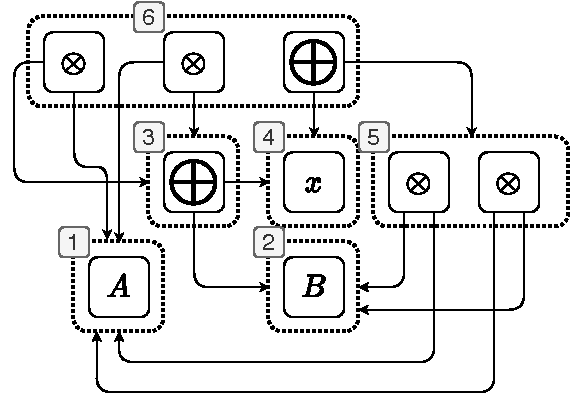
\includegraphics[width=0.45\linewidth]{egraph}
%   \caption{Example \egraph.}\label{fig:eqsat}
% \end{figure}

Throughout the FGH-optimizer we need to manipulate expressions, apply
rules, and manage equivalent expressions.  This problem is common to
all query optimizers.  Instead of implementing our own expression
manager, 
 we again leverage the equality saturation (\eqsat) system 
 as we did in Chapter~\ref{chapter:spores}.
Specifically, we used
egg~\cite{DBLP:journals/pacmpl/WillseyNWFTP21} to implement the green
boxes in the architecture shown in Fig.~\ref{fig:arch}.

% An \eqsat\ system maintains a data structure called an
% \egraph\ that compactly represents a set of expressions, together with
% an equivalence relation over this set.  Each \egraph\ consists of a set
% of \eclasses, each \eclass\ consists of a set of \enodes, and each
% \enode\ is a function symbol with \eclasses\ as children.
% As a refresher, Figure~\ref{fig:eqsat} shows an \egraph\ representing the two
% expressions in Eq.~\eqref{eq:axiom:pullmul}, their subexpressions, and
% other equivalent expressions.  Each \eclass\ (dotted box) represents a class of
% equivalent expressions.  For example \eclass\ 5 represents
% $A \otimes B$ and $B \otimes A$, which are equivalent by
% commutativity.  \eclass\ 6 represents four equivalent expressions
% (including the two choices in \eclass\ 5).

% The \eqsat\ system maintains separately a collection of {\em rules},
% each represented by a pair of patterns.  For example, one rule may
% state that $\otimes$ is commutative: $x \otimes y = y \otimes x$.  The
% \egraph\ can efficiently add a new expression to its collection,
% insert a new rule, and match a given expression against the \egraph.

We describe how we use EGG in the FGH-optimizer.  First, we use it to
extend the Rule-based test (Sec.~\ref{sec:axiomatic-rewrite}) to
account for a constraint $\Gamma$.  By design, the \egraph\ makes it
easy to infer the equivalence $P_1 = P_2$ from a set of rules.
Suppose we want to check such an equivalence conditioned on $\Gamma$.
We may assume w.l.o.g.\ that $\Gamma$ is a logical implication,
$\Delta \Rightarrow \Theta$ since all database constraints are
expressed this way.  We convert it into an equivalence
$\Delta \wedge \Theta = \Delta$, and insert it into the \egraph, then
check for equivalence $P_1 = P_2$.

Second, we use the \egraph\ to denormalize an expression.  More
precisely, recall from Sec.~\ref{subsec:rule:based:synthesis} that we
attempt to synthesize $H$ by denormalizing
$P_1 \defeq \text{normalize}(F(G(X)))$, in other words, writing it in
the form $H(G(X))$.  For that we add $G(X)$ to the \egraph, observe in
which \eclass\ it is inserted, and replace that \eclass\ with a new
node $Y$.  The root of the new \egraph\ represents many equivalent
expressions, and each of them is a candidate for $H$.  We choose the
expression $H$ that has the smallest AST {\em and} does not have any
occurrence of the IDBs $X$.

Finally, we use the \egraph\ to infer the loop invariants.  We do this
by symbolically executing the recursive program $F$ for up to 5
iterations, and compute the symbolic expressions of the IDBs $X$:
$X_0, X_1, \ldots$  Using an \egraph\ we represent all identities
satisfied by these (distinct!) expressions.  The identities that are
satisfied by every $X_i$ are candidate loop invariants: for each of
them we use the SMT solver to check if they satisfy
Eq.~\eqref{eq:invariant:1} from 
Sec.~\ref{subsec:loop:invariants}.

%%% Local Variables:
%%% mode: latex
%%% TeX-master: "main"
%%% End:

\begin{figure*}
    {\small
      \begin{center}
        \begin{tabular}{ l l c c l c } \hline
          Program & Type & Con. & Inv. & Dataset & \required{\#op} \\ \hline
          Beyond Magic (BM) & rule-based & No & Yes & twitter, epinions, wiki & \required{6} \\ 
          Connected Components (CC) & rule-based & No & No & twitter, epinions, wiki & \required{6} \\ 
          Single Source Shortest Path (SSSP) & rule-based & No & No & twitter, epinions, wiki & \required{17} \\ 
          Sliding Window Sum (WS) & \cegis\ & No & Yes & Vector of Numbers & \required{15} \\ 
          Betweenness Centrality (BC) & \cegis\ & No & No & Erdős–Rényi Graphs & \required{43} \\ 
          Graph Radius (R) & \cegis\ & Yes & Yes & Random Recursive Trees & \required{12} \\ 
          Multi-level Marketing (MLM) & \cegis\ & Yes & Yes & Random Recursive Trees & \required{6} \\ \hline
        \end{tabular}
      \end{center}
    }
      \caption{Experimental Setup.
       ``Type'' is the type of synthesis required to optimize the program.
       ``Con.'' means whether the input
        database has constraints. ``Inv.'' means whether optimizing the program
        requires loop invariants.
        ``\#op'' is the number of operations in the program. }
      \label{fig:setup}
    \end{figure*}
    
    \begin{figure*}
      \centering
      \begin{subfigure}[b]{0.48\textwidth}
        \centering
        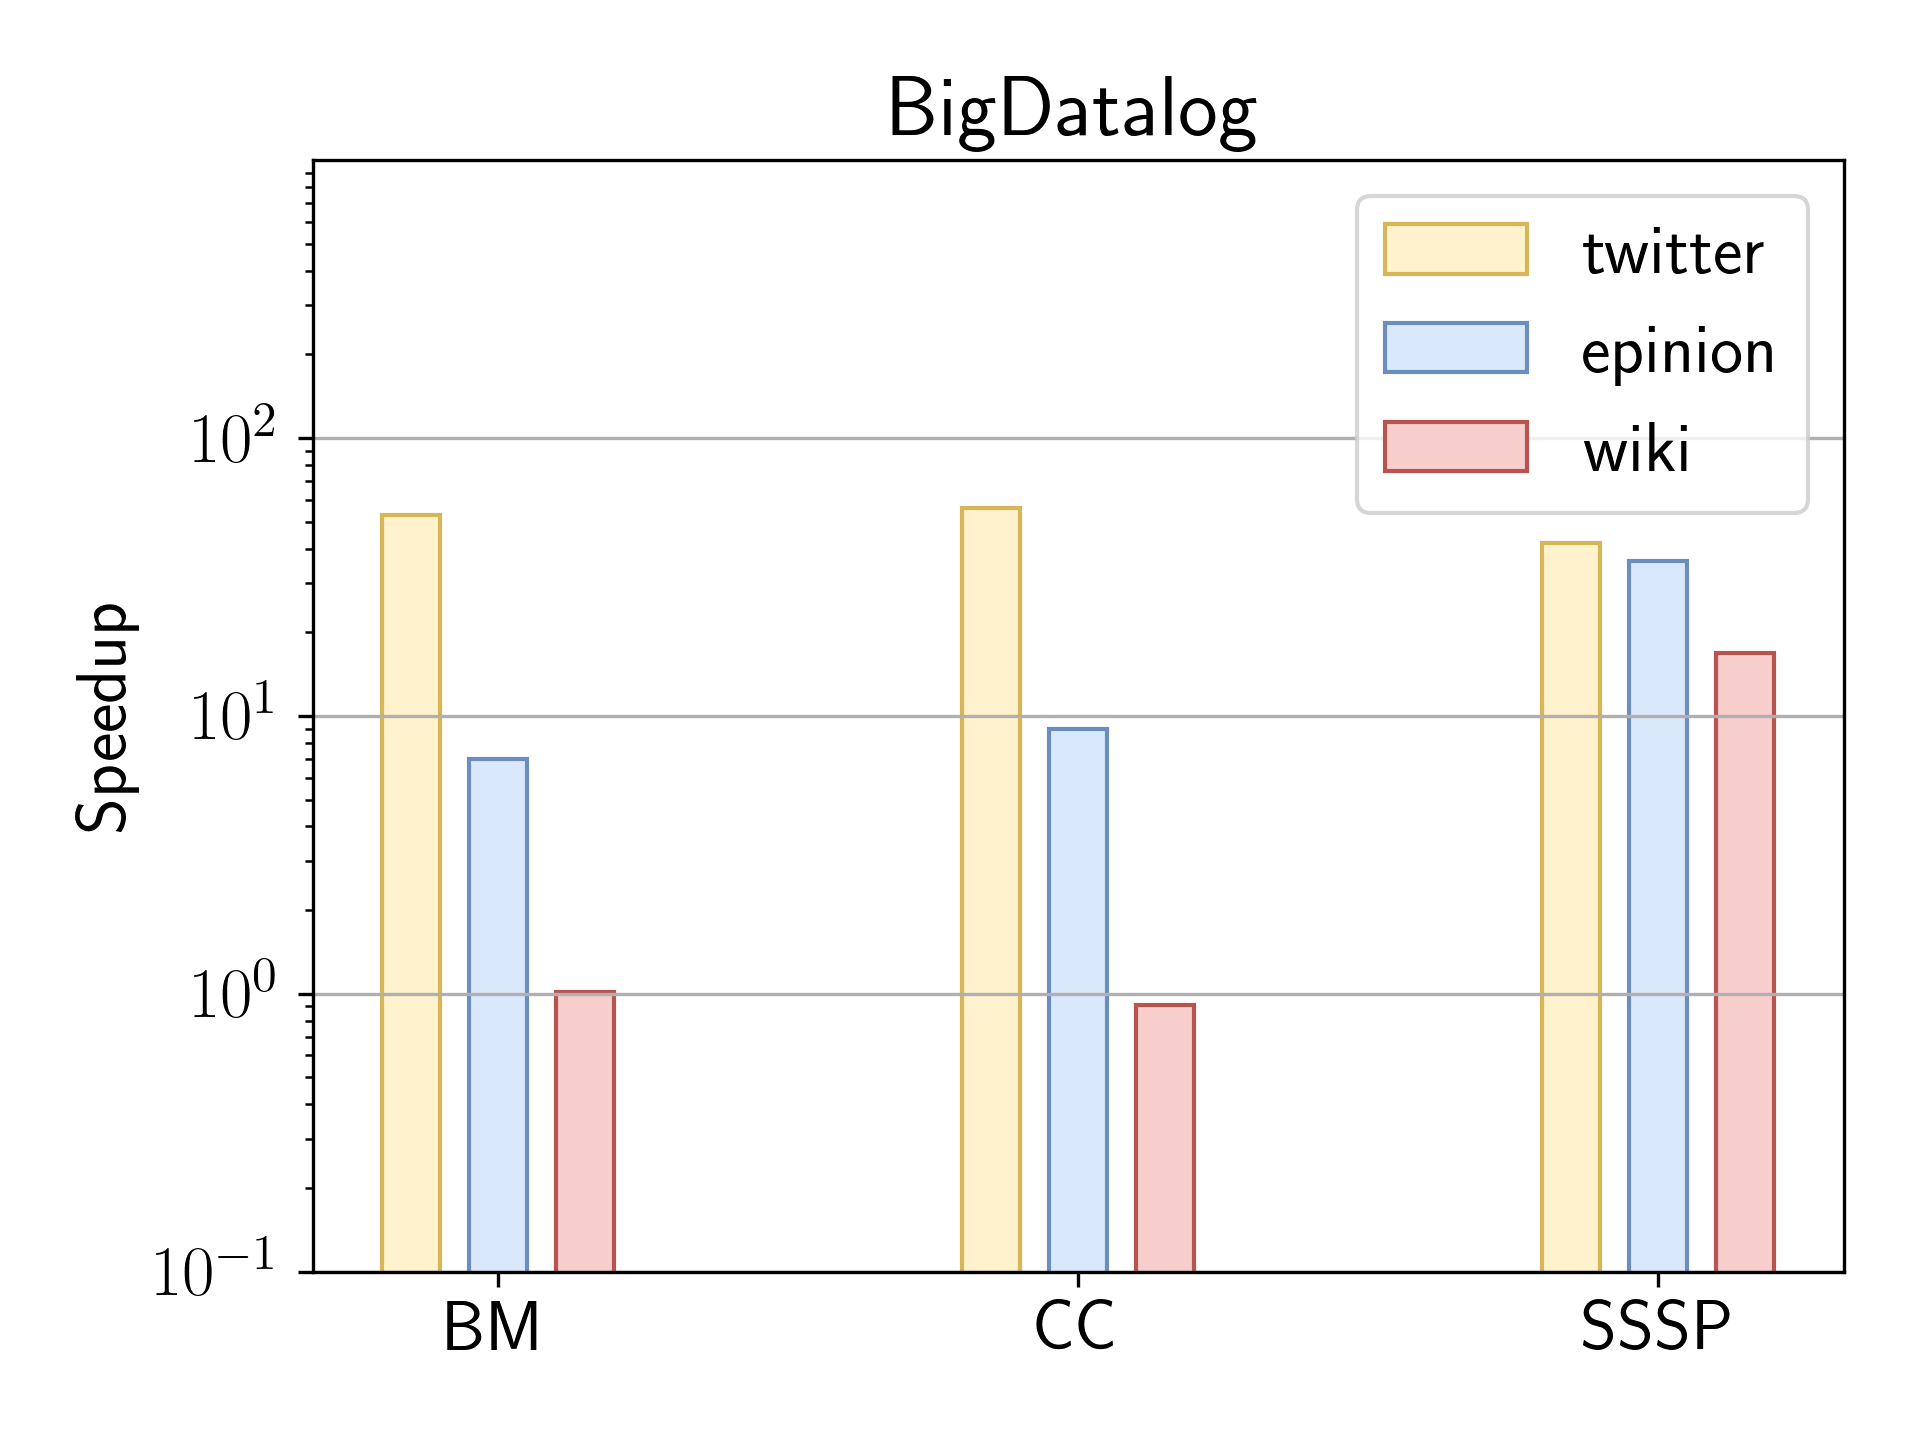
\includegraphics[width=\textwidth]{basic-bd}
        % \caption{BigDatalog}\label{fig:eval:basic:bd}
      \end{subfigure}

      \begin{subfigure}[b]{0.48\textwidth}
        \centering
        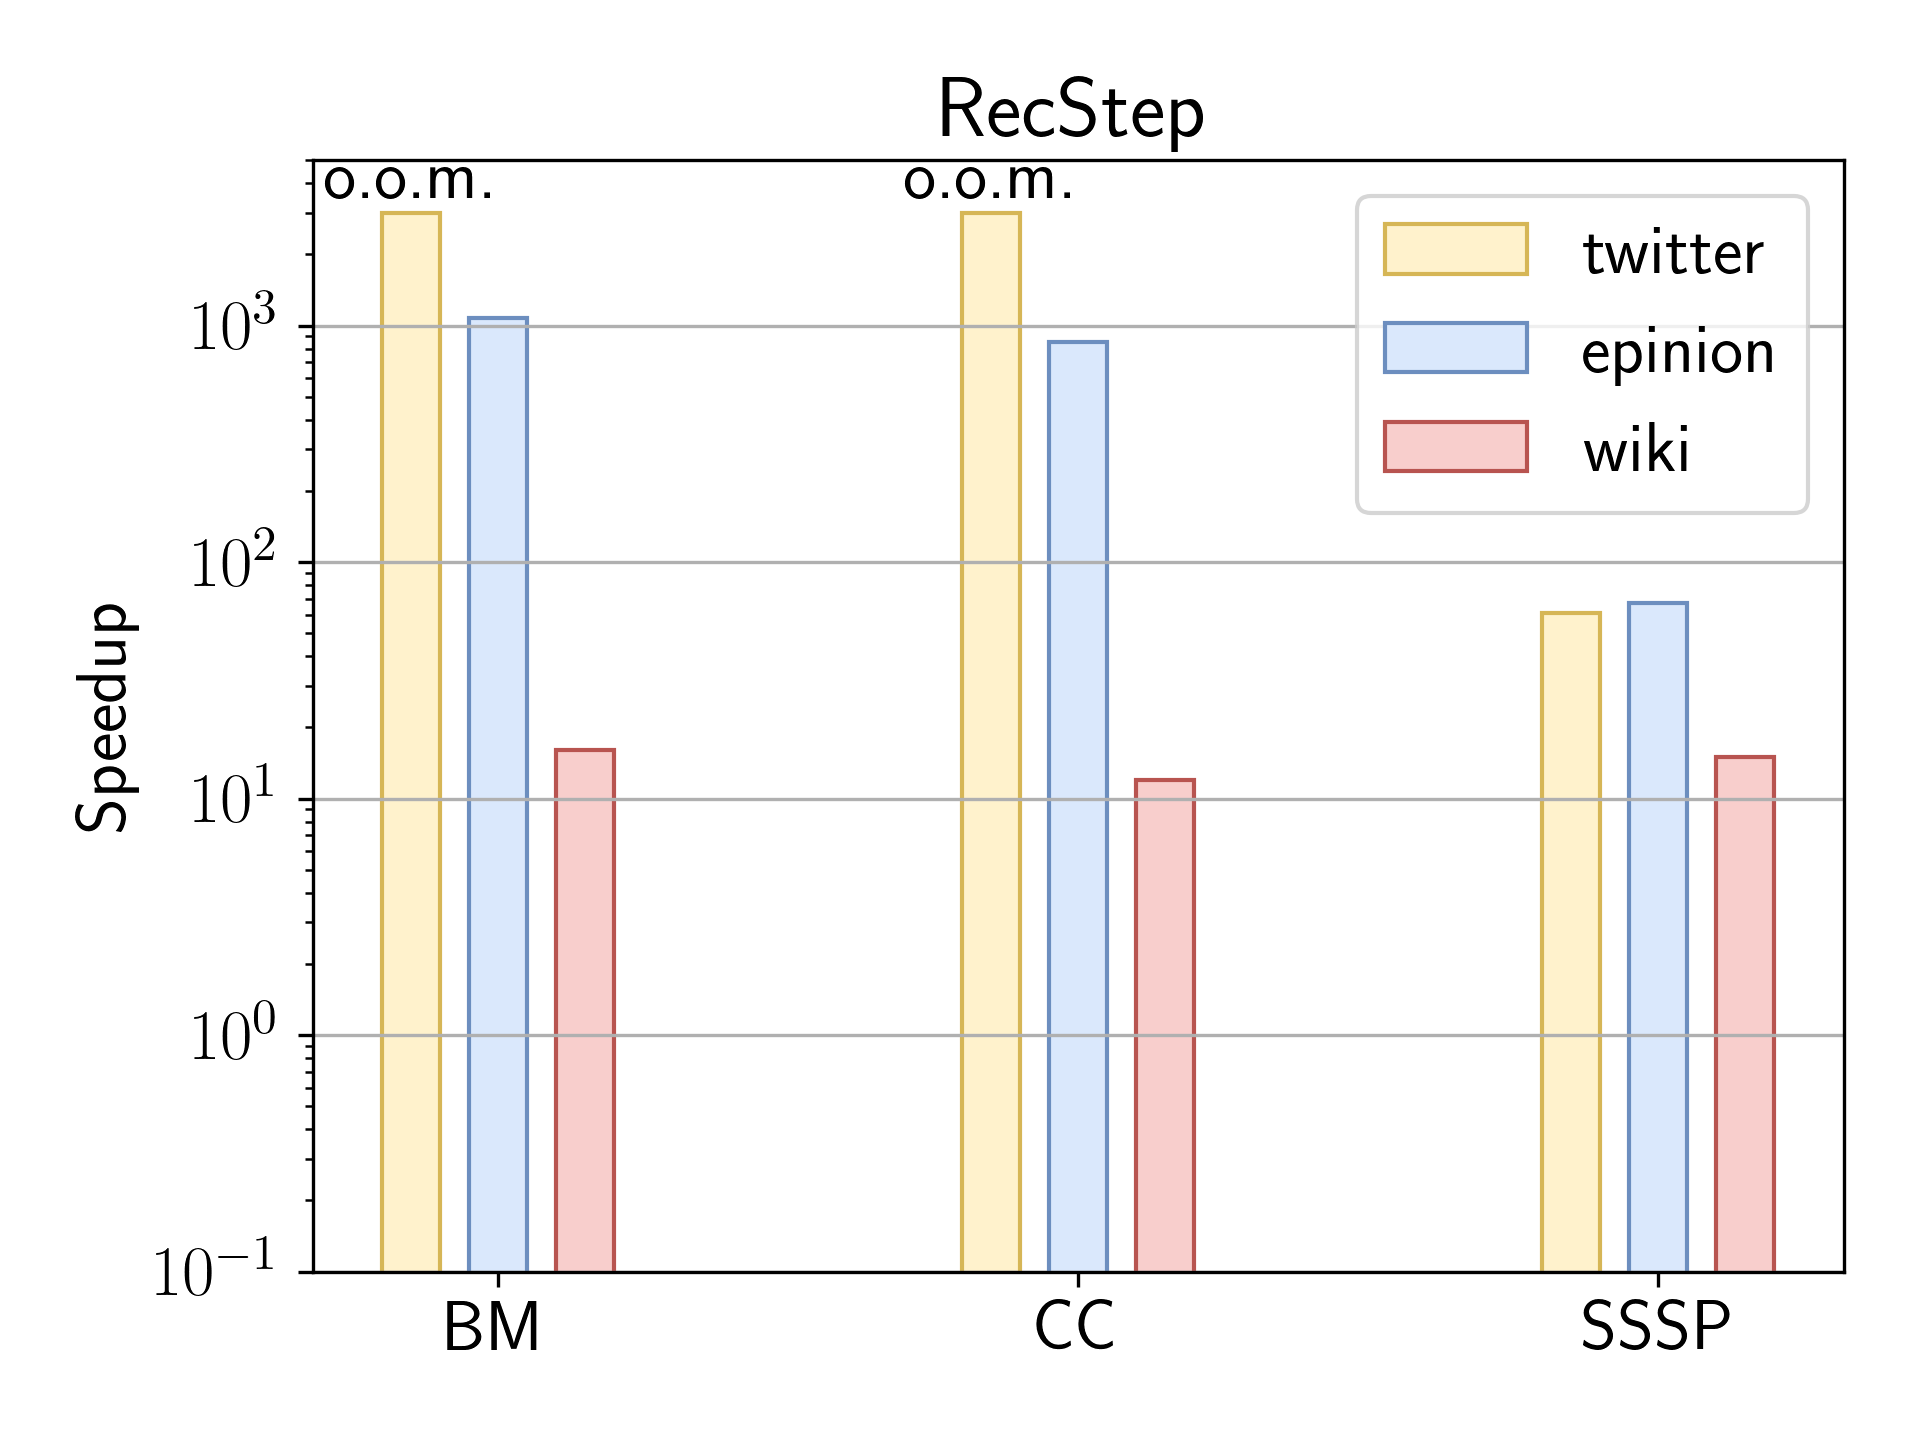
\includegraphics[width=\textwidth]{basic-rs}
        % \caption{RecStep}\label{fig:eval:basic:rs}
      \end{subfigure}
      \hfill
      \begin{subfigure}[b]{0.48\textwidth}
        \centering
        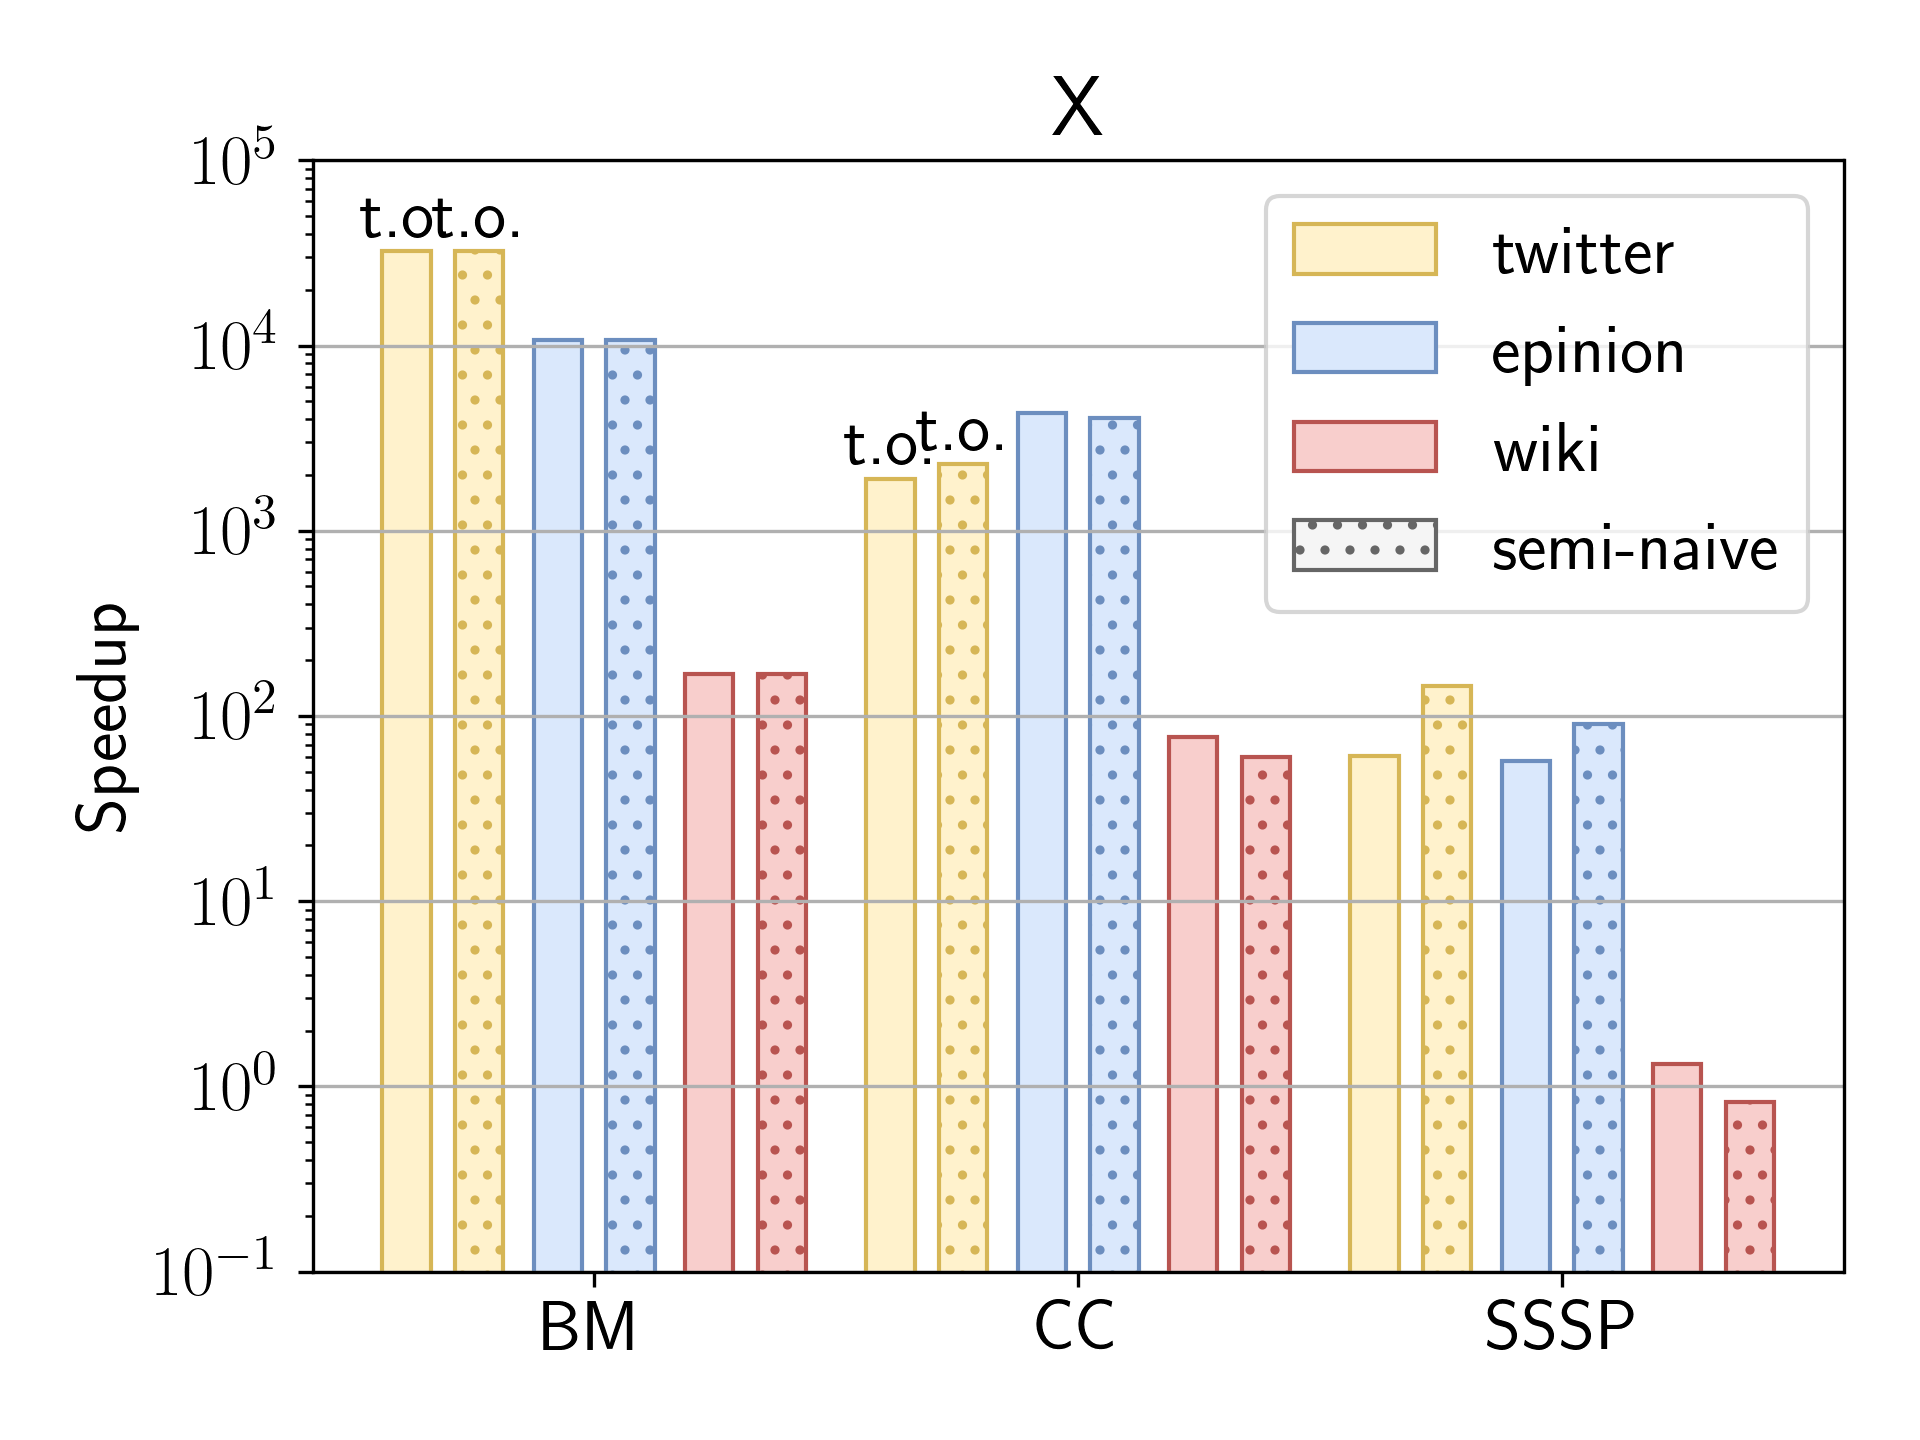
\includegraphics[width=\textwidth]{basic-x}
        % \caption{X}\label{fig:eval:basic:x}
      \end{subfigure}
      \caption{Speedup of the optimized v.s.\ original program; higher is better; 
      \required{t.o. means the original program timed out after 3 hours, in which case we report the speedup against 3 hours; o.o.m. means the original program ran out of memory.}}\label{fig:eval:eqsat}
    \end{figure*}
    
    \begin{figure*}
        \centering
        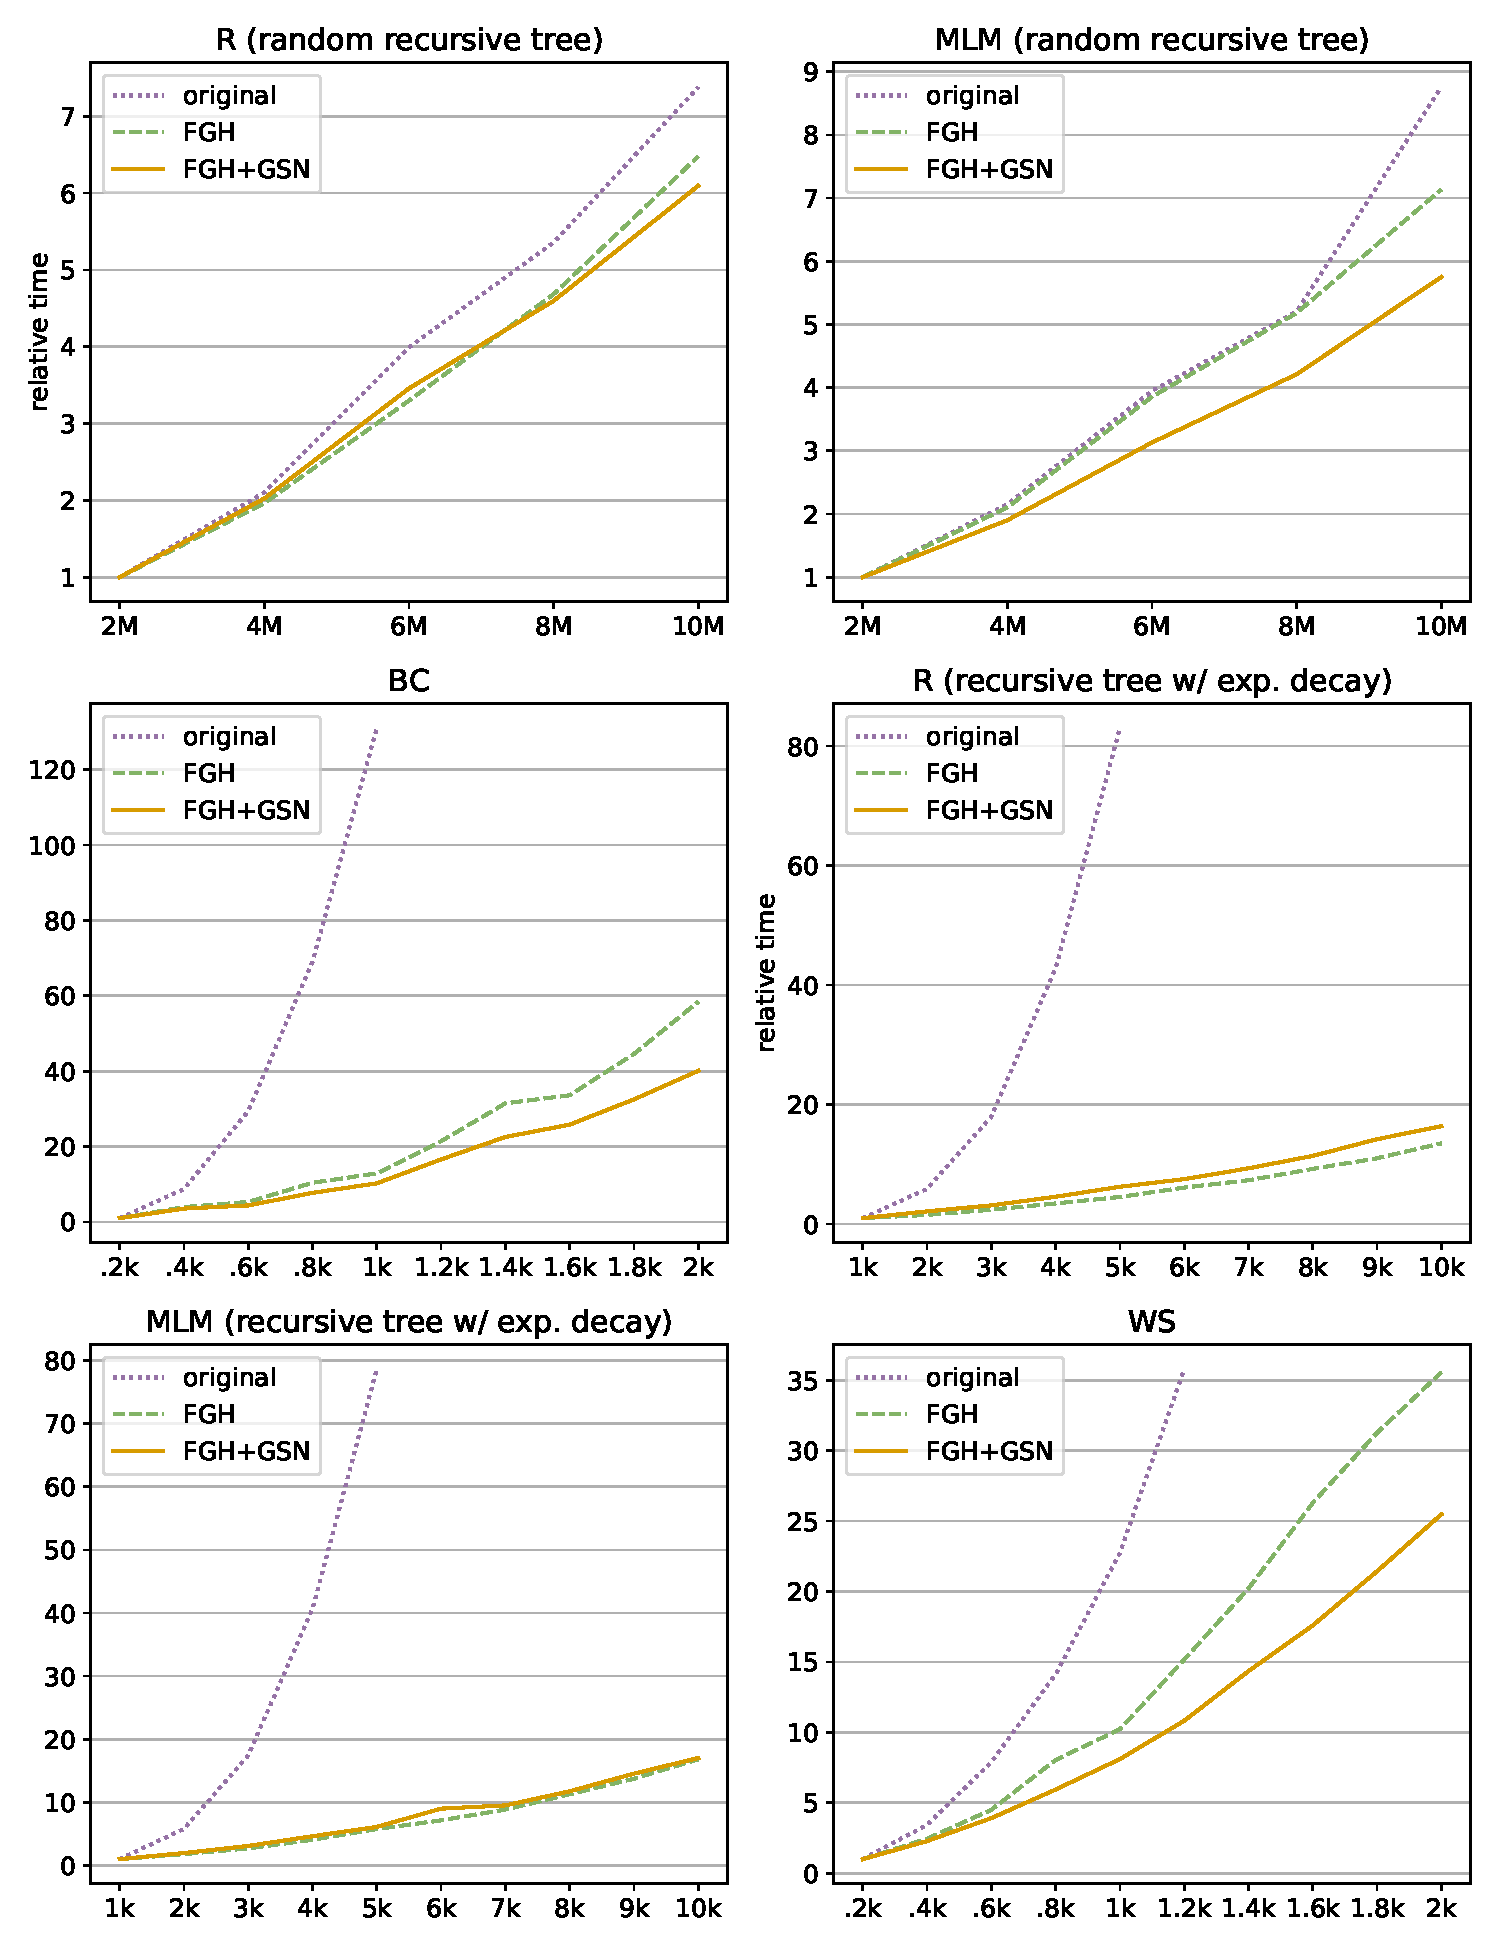
\includegraphics[width=\textwidth]{hard_bench}
        \caption{Runtime increase as a function of the data size; lower is  better.}\label{fig:eval:hard}
    \end{figure*}
    
    \begin{figure*}
      \centering
     \begin{tabular}{ c | c c c | c c c c }
     Program & BM & CC & SSSP & R & MLM & BC & WS \\
     \hline
     Invariance inference & 0.092 & 0 & 0 & 0.129 & 0.132 & 0 & 0\\
     Synthesis & 0.004 & 0.005 & 0.004 & 0.284 & 0.299 & 1.2 & 0.821 \\
     \hline
     Total & 0.096 & 0.005 & 0.004 & 0.413 & 0.431 & 1.2 & 0.821 \\
     Opt. / Exec. (max\%-min\%) & .82 - .16 & .04-.01 & .24-.002 & .41-.07 & .76-.09 & 6.3-.51 & 7.4-.66
    \end{tabular}

    \vspace{1em}

    \begin{tabular}{ c | c c c c }
     Program & R & MLM & BC & WS \\
     \hline
     Search space & 10 & 20 & 132 & 94 \\
    \end{tabular}
      \caption{Optimization time in seconds, 
      \required{optimization time over execution time,}
       and  size of the search space. }
      \label{fig:synthesis:time:space}
    \end{figure*}
    
    \section{Evaluation}\label{sec:eval}
    
    We implemented a source-to-source FGH-optimizer, based on
    Fig.~\ref{fig:arch}.  The input is a program $\Pi_1$, given by $F, G$,
    and a database constraint $\Gamma$, and the output is an optimized
    program $H$.  We evaluated it on three Datalog systems, and several
    programs from benchmarks proposed by prior
    research~\cite{BigDatalog, DBLP:journals/pvldb/FanZZAKP19}; we also
    propose new benchmarks that perform standard data analysis tasks.  We
    did not modify any of the three Datalog engines.  We asked two major
    questions:
    \begin{enumerate}
    \item How effective is our source-to-source optimization, given that
      each system already supports a range of optimizations?
    \item How much time does the actual FGH optimization take?
    \end{enumerate}
    
    \subsection{Setup}
    
    % \dan{Remy: we need 2-3 sentences explaining why you ended up with
    %   these systems, and examples of other systems that you considered but
    %   couldn't use}
    
    There is a great number of commercial and open-source Datalog engines in the
    wild, but only a few support aggregates in recursion.
    % Supporting non-recursive
    % aggregate is straightforward given any  Datalog engine: simply create a separate
    % stratum for the aggregation. Therefore, we only consider one system that lacks
    % recusive aggregate and use it as a baseline.
    We were able to identify five major systems with such support:
    SociaLite~\cite{DBLP:journals/tkde/SeoGL15},
    Myria~\cite{10.14778/2824032.2824052}, the DeALS family of systems
    (DeALS~\cite{DBLP:conf/icde/ShkapskyYZ15},
    BigDatalog~\cite{DBLP:conf/sigmod/ShkapskyYICCZ16}, and
    RaDlog~\cite{DBLP:conf/sigmod/0001WMSYDZ19}),
    RecStep~\cite{DBLP:journals/pvldb/FanZZAKP19}, and
    Dyna~\cite{francislandau-vieira-eisner-2020-wrla}.
    Prior work~\cite{BigDatalog} reports SociaLite and Myria are consistently slower than
    newer systems, so we do not include them in our experiments.
    Dyna is designed to experiment with novel language semantics and
    not for data analytics, and we were not able to run our benchmarks
    without errors using it.
    Systems in the DeALS family are similar to each other;
    we pick BigDatalog because it is open source
    and runs our benchmarks without errors;
    we include RecStep for the same reasons.
    Both BigDatalog and RecStep are multi-core systems.
    Finally, we run experiments on an unreleased commercial system X,
    which is single core.
    As we shall discuss, X is the only one that supports all features for
    our benchmarks.
    
    We conducted all experiments on a server running CentOS 8.3.2011.
    The server has a total of 1008GB memory, and
    4 Intel Xeon CPU E7-4890 v2 2.80GHz CPUs, 
    each with 15 cores and 30 threads. 
    We ran seven
    benchmarks, shown in Fig~\ref{fig:setup}. BM and CC are
    Examples~\ref{ex:more:magic} and ~\ref{ex:fgh:cc}; MLM is basically
    Example~\ref{ex:fgh:constraints}.  CC, SSSP and MLM are
    from~\cite{BigDatalog}, the others are designed by us.  R and MLM
    require a database constraint stating that the data is a tree.  BM,
    R, and MLM each have a non-trivial loop invariant that is inferred by the
    optimizer.  
    \required{Our optimizer requires each program to consist of two rules,
    one each for $F$ and $G$, and so a meaningful metric for
    program size is the number of semiring operations.
    These numbers are listed in the last column of Fig~\ref{fig:setup}.
    Our benchmark programs are comparable in size to those used in prior work~\cite{BigDatalog, DBLP:journals/pvldb/FanZZAKP19}.}
    All programs are available in our git repository.  The
    real-world datasets twitter~\cite{mcauley2012learning}, epinions~\cite{richardson2003trust}, and
    wiki~\cite{leskovec2010signed} are from the popular SNAP collection~\cite{snapnets}.  We
    follow the setting in~\cite{BigDatalog,DBLP:journals/pvldb/FanZZAKP19}
    when generating the synthetic graphs.
    We additionally generate random recursive trees with an exponential
    decay, modeling the decay of association in multi-level
    marketing~\cite{emek2011mechanisms}.
    For WS, we input the vector
    $[1, \ldots, n]$, since the values of the entries do not affect run time.
    In general, we used smaller datasets
    than~\cite{BigDatalog,DBLP:journals/pvldb/FanZZAKP19} because some of
    our experiments run single-threaded.
    
    
    
    
    
    \subsection{Run Time Measurement}
    
    %%% We measure the run time of Datalog programs drawn from benchmarks
    %%% proposed by prior research~\cite{BigDatalog, DBLP:journals/pvldb/FanZZAKP19};
    %%% we also propose new benchmarks that perform standard data analysis tasks.
    %%% We run the programs on real-world datasets drawn from popular
    %%% benchmarks as well as synthetic data.
    %%% The following table lists these programs and datasets:
    %%% 
    %%% The programs TC, CC, SSSP and MLM are drawn from~\cite{BigDatalog}.
    %%% We divide the programs into two groups in the table above:
    %%% the first group of 3 programs can each be optimized by the basic FGH-rule;
    %%% in other words, they require only rewriting (\eqsat) and not synthesis.
    %%% The second group of 4 require synthesis (\cegis);
    %%% programs R and MLM contain the integrity constraint
    %%% that the input is a tree.
    
    For each program-dataset pair, we measure the run times of three
    programs: original, with the FGH-optimization, and with the
    FGH-optimization and the generalized semi-naive (GSN, for short)
    transformation.  We report only the speedups relative to the original
    program in Fig.~\ref{fig:eval:eqsat} and~\ref{fig:eval:hard}.  In some
    cases the original program timed out our preset limit of 3 hours, 
    \required{where we report the speedup against the 3 hours mark.
    In some other cases the original program ran out of memory and we mark them with ``o.o.m.'' in the figure.
    }  The {\em absolute} runtimes are irrelevant
    for our discussion, since we want to report the effect of {\em adding}
    our optimizations.  (We also do not have permission to report the
    runtimes of X.)  All three systems already perform semi-naive
    evaluation on the original program, since that is expressed over the
    Boolean semiring.  But the FGH-optimized program is over a different
    semiring (except for BM), and GSN has non-stratifiable rules with
    negation, which are supported only by system X; we report GSN only for
    system X.  While the benchmarks in Fig.~\ref{fig:eval:eqsat} were on
    real datasets, those in Fig.~\ref{fig:eval:hard} use synthetic data,
    for multiple reasons: we did not have access to a good tree dataset
    needed in the R and MLM benchmarks, BC timed out on our real data (BC
    is computationally expensive), and WS uses only a simple array.  A
    benefit of synthetic data is that we can report how the optimizations
    scale with the data size.  Unfortunately, the FGH-optimized programs
    in Fig.~\ref{fig:eval:hard} require recursion with \textsf{SUM}
    aggregation, which is not supported by BigDatalog or RecStep; this is
    in contrast with those in Fig.~\ref{fig:eval:eqsat}, which require
    recursion with \textsf{MIN} aggregation which is supported by all
    systems.
    
    % before and after optimization; when applicable, we also measure the
    % speedup with and without generalized semi-naive transformation (GSN,
    % for short).  Note that expressing GSN requires non-monotone rules and
    % non-stratifiable negation.  At the time of writing only X supports
    % both of these features.  BigDatalog and RecStep also do not support
    % recursive \textsf{SUM}, which is necessary for the FGH-optimized
    % programs BC and MLM.  For these reasons we run the second group of
    % benchmarks on X only.  We cannot report the raw run time of X, and
    % since the experiments are not meant to compare the systems against
    % each other, we only report speedup and relative time.
    
    
    \subsubsection{Findings} Figure~\ref{fig:eval:eqsat} shows the results
    of the first group of benchmarks optimized by the
    rule-based synthesizer.  Overall, we observe our optimizer provides
    consistent and significant (up to 4 orders of magnitude) speedup across
    systems and datasets.  Only a few datapoints indicate the optimization
    has little effect: BM and CC on wiki under BigDatalog, and SSSP on
    wiki under X.  This is due to the small size of the wiki dataset: both
    the optimized and unoptimized programs finish very quickly, so the run
    time is dominated by system overhead which cannot be optimized away.
    We also note that (under X) GSN speeds up SSSP but slows down CC (note the log scale).
    The latter occurs because the $\Delta$-relations for CC are very large,
    and as a result the semi-naive evaluation has the same complexity as
    the naive evaluation; but the semi-naive program is more complex and
    incurs a constant slowdown.  GSN has no effect on BM because the
    program is in the boolean semiring, and X already implements the
    standard semi-naive evaluation.
    Optimizing BM with FGH on BigDatalog sees a significant speedup even though the
    systems already implements magic set rewrite,
    because the optimization depends on a loop invariant.\footnote{
    BigDatalog can optimize the left-recursive version of BM~\eqref{eq:simple:magic:nonopt}
    to obtain similar speedup, via the classic magic set rewrite.}
    Overall, both the semi-naive and
    naive versions of the optimized program are significantly faster than
    the unoptimized program.
    
    Figure~\ref{fig:eval:hard} shows the results of the second group of
    benchmarks, which required \cegis.  Since we used synthetic data,  we
    examined here the asymptotic behavior of the optimization as a
    function of the data size.
    % The programs in this group are
    % more complex and take longer to run, so we limit our data size to
    % ensure the experiments finish in reasonable time.  
    The most advanced optimization was for BC, which leads essentially to
    Brandes' algorithm~\cite{brandes2001faster}: its effect is dramatic.
    R and MLM rely on semantic optimization for a tree.  We generated two
    synthetic trees, a random recursive tree with expected depth of
    $O(\log n)$ and one with exponential decay with expected depth of
    $O(n)$.  Since the benefit of the optimization depends on the depth,
    we see a much better asymptotic behavior in the second case.  Here,
    too, the optimizations were always improving the runtime.
    
    % 
    % 
    % Overall, we observe weak asymptotic speedup for R and MLM on random
    % recursive trees, and strong asymptotic speedup in all other cases.
    % Recall programs R and MLM constrain their input to be trees.  For the
    % two programs, the optimized programs are only slightly faster than the
    % unoptimized one.  Closer examination of the optimized code reveals
    % similar complexity as the unoptimized one.  For example, the original
    % MLM first computes the transitive closure of size $O(n\log(n))$ where
    % $n$ is the size of the tree.  This only leaves a $\log(n)$ factor to
    % be optimized away, so the optimized programs are not much faster
    % despite requiring only linear space.  The speedup becomes much more
    % pronounced when we introduce exponential decay when generating the
    % random trees.  Then the trees are much deeper (with $\Omega(n)$
    % depth), which forces the transitive closure in the unoptimized program
    % to take space $\Omega(n^2)$, whereas the optimized programs still run
    % in linear space.
    % % Notably, the programs run slightly slower under semi-naive evaluation. 
    % % This is also caused by the large depth of the tree:
    % % the higher nodes are shared by many paths to the root, 
    % % and will be repeatedly updated with new deltas throughout semi-naive
    % % evaluation. 
    % For BC and WS, the naive version of
    % the optimized program already speeds up the program significantly, and
    % the semi-naive version contributes further speedup.  
    % 
    
    % \reinhard{Is it clear what SN and OG in  Figure~\ref{fig:eval:hard}  mean? Should SN be replaced by GSN? What about OG?}
    
    \subsection{Optimization Time and  Search Space}
    
    \cegis\ can quickly become very expensive if its search space is
    large, and, for that reason, we have designed the grammar generator
    carefully to reduce the search space without losing generality.
    Fig.~\ref{fig:synthesis:time:space} reports the runtime of the
    synthesizer (in seconds) for both rule-based synthesis and \cegis, and the size
    of the search space.  The rule-based synthesizer runs in
    milliseconds, while \cegis\ took over 1s for BC (our hardest
    benchmark).  These numbers are close to those demanded by modern query
    optimizers, and represent only a tiny portion of the total runtime
    of the optimized query. 
    \required{
    Optimization time takes less than 1\% of the query run time for all benchmarks except for BC and WS on the smallest input data. }
    To our surprise, our grammar managed to
    narrow the search space considerably, to no more than 132 candidates,
    which (in hindsight) explains the low optimization times. 
    \required{
    The search space can grow rapidly, and even exponentially, 
    as the size of the input program grows.
    Our optimizer optimizes a single stratum at a time, 
    focusing on improving critical ``basic blocks'' of a program.
    Our benchmark programs demonstrate a wide range of data analysis computation can
    be expressed succinctly using just a few semiring operations, 
    and optimization can have a dramatic impact on performance.}
    
    \subsection{Summary}
    
    We conclude that our optimizer can significantly speedup already
    optimized  Datalog  systems, either single-core or multi-core.  GSN
    can, sometimes, further improve the runtime.  We achieved this using a
    rather small search space, which led to fast optimization.
    
    
    % programs across different execution engines and datasets.  In some
    % cases, GSN is necessary to achieve the best performance; in other
    % cases GSN has no effect or even slightly slows down the optimized
    % program.  Since the GSN transformed programs are almost always faster
    % than the baseline, we argue it should be implemented in future Datalog
    % systems.
    % 
    % \reinhard{Wouldn't it be nicer if we could conclude by emphasizing the benefit of {\em our} optimization 
    % rather than of GSN (or at least mention that the combination of the two is unbeatable)?}
    
    % \subsection{Compilation Time}
    % Figure~\ref{fig:synthesis:time:space} shows the compile time breakdown
    % for each program.
    % %
    % \reinhard{Should we state that the numbers in the table are to be understood as 
    % ``percent relative to the run time of the unoptimized program''?}
    % %
    % Overall, compilation takes under $1\%$ of the total
    % run time of the unoptimized program.
    % All programs from the first group are compiled faster than those from the
    % second.
    % This is because optimizing the first group does not require synthesis
    % and only involves \eqsat, which is very fast.
    % In our implementation we invoke invariant inference on demand.
    % That is, we first attempt optimization without invariants,
    % and only when this fails do we invoke invariant inference.
    % Since optimizing CC, SSSP, BC and WS does not require invariants,
    % we skip the inference step.
    % 
    
    
    %%% Local Variables:
    %%% mode: latex
    %%% TeX-master: "main"
    %%% End:

    % \section{Summary and Discussion}